\begin{savequote}
``Even though the computer code may be free of error to the extent that it operates exactly as its author intended, it is seldom possible to give a rigorous proof that these intentions were correct.''
\qauthor{P.L.Roe, Ann. Rev. Fluid Mech. 1986 18:337-65}
\end{savequote}



\chapter{Numerical Tests}
%Testing the code}
%\minitoc

In this Chapter the method for testing the performance of the code against
experimental data and standard tests from the literature is outlined. The various
tests are described.
These include tests for problems in pure hydrodynamics and magnetohydrodynamics
in one and two dimensions, also a test for the perfomance of the radiative
cooling algorithm in the code.
The code comparison between ATLAS and the PLUTO code for problems relevant to
astrophysics is also described.

\section{Introduction}
%Verification and validation of codes is increasingly important as they are the main tools for understanding the complexities of the observed universe.
% It is impossible to ensure that the code will always be right - but can check the calculations.
It is not possible to ensure that any numerical code will provide a meaningful physical solution with arbitrary input but it is possible to establish confidence by \emph{verifying} numerical calculations against 
\begin{itemize}
\item experimental results
\item analytical solutions 
\item results of other numerical calculations.
\end{itemize}

The process of \emph{verification} is informally defined as  ``solving the equations right'' \citep{1976cfd..book.....R}.

The complementary procedure of \emph{validation} is defined as ``solving the right equations'' \citep{1976cfd..book.....R}.
% Otherwise risk invalidating results
%As has been demonstrated \citep{2002ApJ...577L.123F} it is essential to thoroughly test a code before it is used to test new models of physics.
%\citet{2002ApJ...577L.123F} has shown the terrible effect of omitting some tests even on a well-established code.
A suite of standard tests has been built up over the past history of computational physics.
\citet{Sod78:_a_surv} compiled a set of tests for 1D HD shocks.
\citet{1982ApJ...261..543C} tested radiative cooling.
\citet{1988JCoPh..75..400B} extended Sod's work to include MHD.
\citet{Toro:1997:RSN} extended Sod's work to more exacting tests of HD shock-capturing.
\citet{1995ApJ...442..228R} performed tests for multidimensional MHD flow.
\citet{Toth96:_compar} performed algorithm comparisons for HD and MHD problems.
\citet{1998ApJ...494..317D} tested their algorithm in one and two dimensions.
\citet{2003_liska_wendroff} provided more tests in 2D HD.
The most important features of the ATLAS code are how it handles HD and MHD shocks in all directions, with and without radiative cooling.
To test this, the following tests are implemented; shock tube tests, the overstable radiative shock, the double Mach reflection test and the Orszag-Tang vortex are implemented.
Finally a code comparison is made with the astrophysics code PLUTO \citep{2004Ap&SS.293..199M}.
In Table \ref{tab:test} we show a test matrix for ATLAS.




\begin{table}
\begin{tabular}{|p{3.5cm}|p{3.5cm}|p{3.5cm}|p{3.5cm}|}
\hline
& HD  & Cooling & MHD  \\
\hline
1D & Shock Tube & Overstable Shock  & Shock Tube \\
\hline
2D & Mach Reflection & Jet  & Orszag Tang \\
 & Blast & -  & Blast \\
%\hline
%3D & Blast & Jet  & Blast \\
\hline
\end{tabular}
\caption{A Test Matrix for Shock-capturing codes}
\label{tab:test}
\end{table}


\section{HD Tests}


\subsection{One-dimensional Shock Tube}

All shock tube tests were carried out using a grid of 500 cells in size, a Courant number of 0.5 and an adiabatic index of $\gamma=5/3$.
This test was taken from Laney, contains an expansion fan which is a good test of the Roe Riemann solver, a contact discontinuity and a shock.
\\Left State:
\begin{equation}
U_L = \left( 
\rho = 1,
v_x =0,
v_y = 10,
p = 20
\right)
\end{equation}
\\Right State:
\begin{equation}
U_R = \left( 
\rho = 1,
v_x = 1,
v_y = -10,
p = 1
\right)
\end{equation}


\begin{figure}[t]
\centering
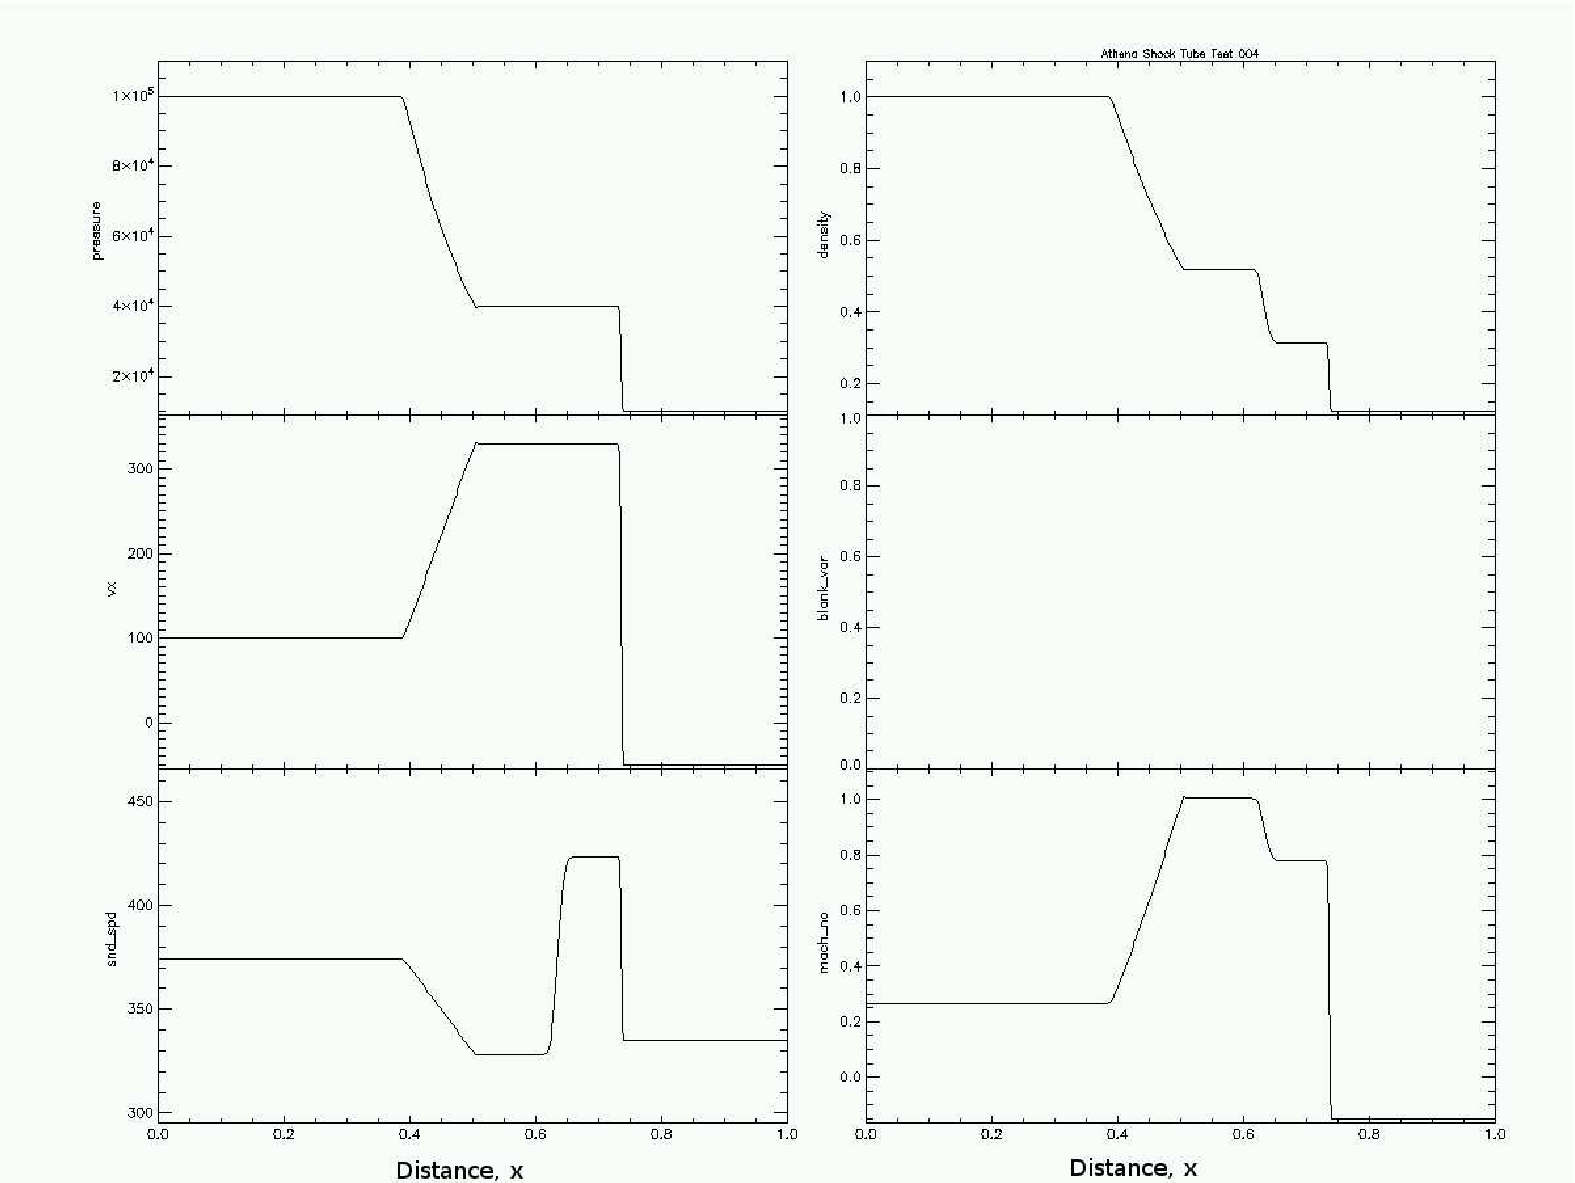
\includegraphics[width=\textwidth]{one_d_hd_shocktube}
\caption{Results of one-dimensional HD shock tube test at time t=0.8 for comparison with \citet{Laney:1998}
Left panels show pressure, velocity, and sound speed. Right panels show density, entropy and Mach number.
The simple features of the expansion fan, contact discontinuity, and shock have all been captured.
}
\label{fig:3-1} % Give a unique label
\end{figure}

\subsection{Blast Wave}

Pure hydrodynamic blast wave test for comparison with \citet[][hereafter LDZ]{2000ApJ...530..508L}.
This test has as its initial conditions a high pressure region in the centre of a plane.
The results are shown in Figure \ref{fig:3-hdblastwave}.
Here the important features are symmetry, correct wave speed evaluation, well-resolved shocks and preservation of the shape of the circular blast wave.

\begin{figure}[t]
\centering
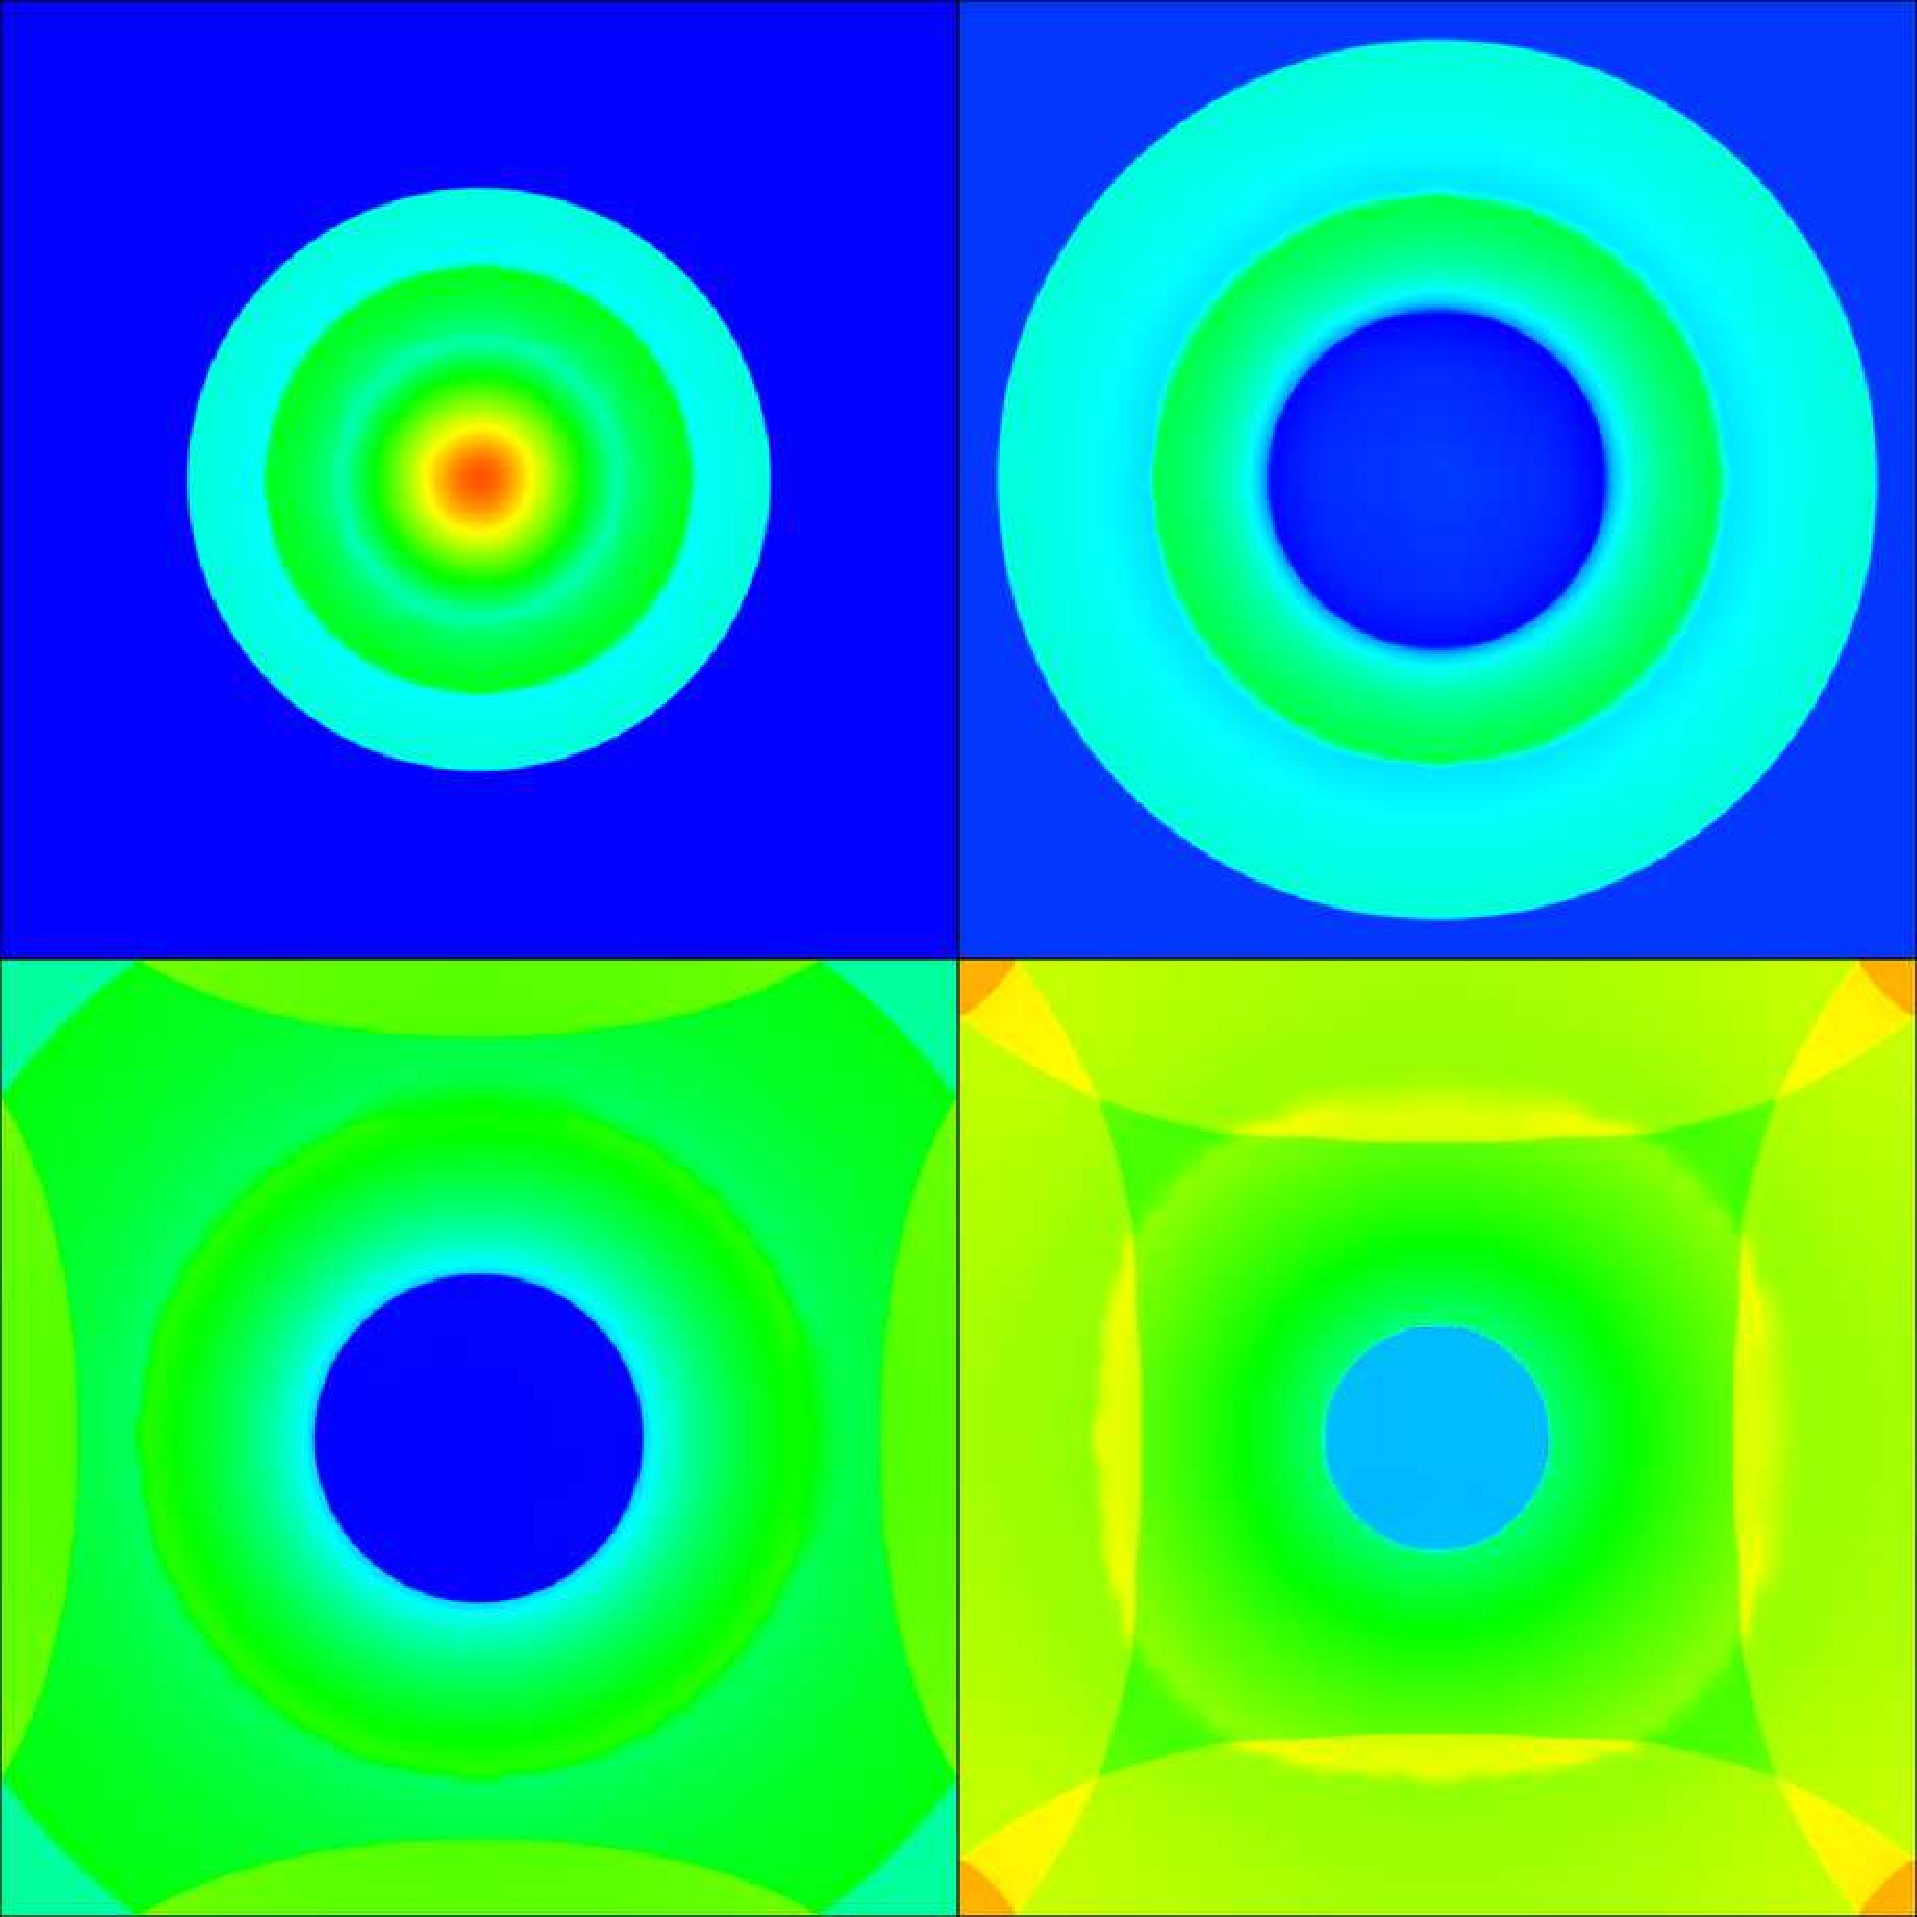
\includegraphics[width=0.9\textwidth]{hdblastwave}
\caption{
The most important feature of the 2D blast wave test is its perfect symmetry. The shock is also well-resolved.
Density colourmaps at times: t=3, 6, 9, 12.
The units are arbitrary.
}
\label{fig:3-hdblastwave} % Give a unique label
\end{figure}

\subsection{Double Mach Reflection (DMR) Test}


\subsubsection{Initial Conditions}

\begin{figure}[t]
\centering
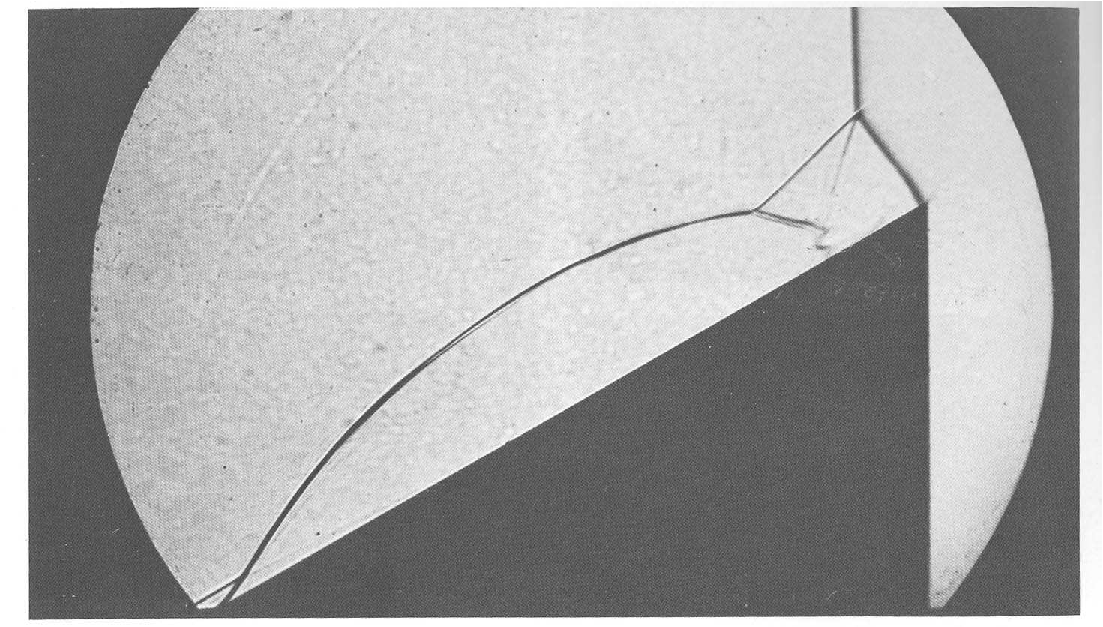
\includegraphics[width=0.8\textwidth]{dmr_experimental}
\caption{
%Double Mach Reflection Experimental Result
A strong shock striking a reflecting wedge gives rise to a complicated pattern of shocks and contact discontinuities. Photograph taken from \citet{1964VanDyke}.
}
\label{fig:DMRExperimental} % Give a unique label
\end{figure}


\begin{figure}[t]
\centering
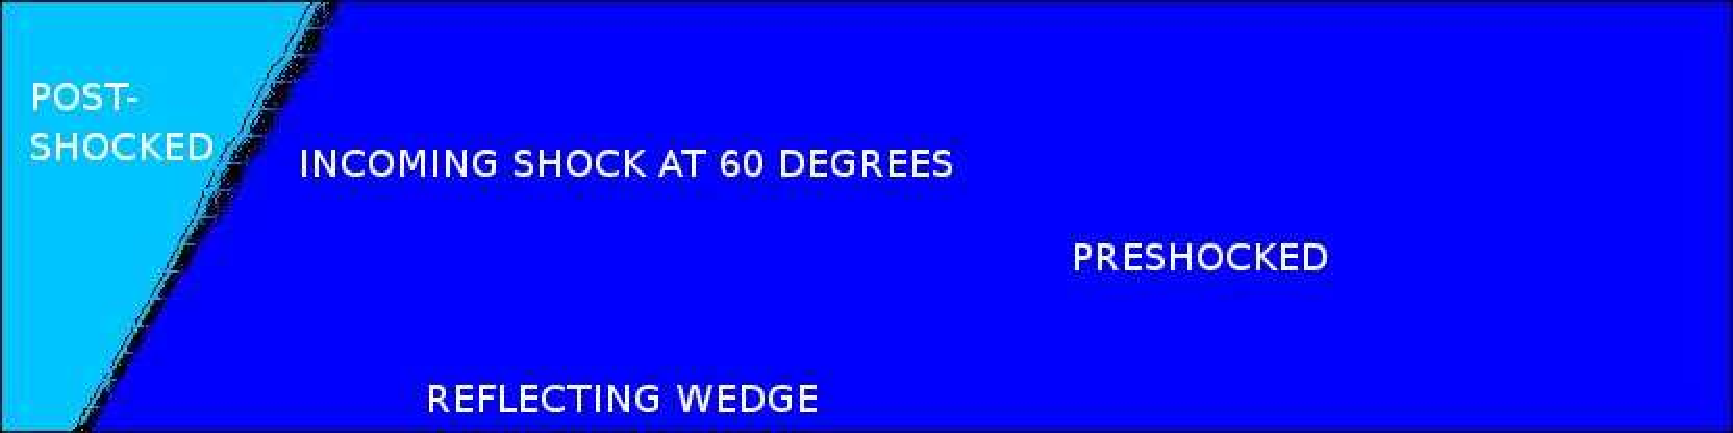
\includegraphics[width=0.8\textwidth]{dmr_initial_conditions}
\caption{
Double Mach Reflection Initial Conditions.
}
\label{fig:DMRInitial} % Give a unique label
\end{figure}

A strong shock incident on reflecting wedge at an angle greater than the critical angle $\phi_{crit}$ will separate into a parallel component and a convex reflected component. 
The three shocks, (incident, parallel and reflected) meet at a point called the triple or lambda point \citep{1959flme.book.....L}. (The figure is thought to resemble the lower-case Greek letter lambda.)
The complicated non-linear reflection and Mach stem formed during the double Mach reflection of a strong shock plus the Kelvin-Helmholtz instabilities which form along the contact discontinuity provides a challenging problem for the numerical code.
It can be reduced to three parameters, $\gamma$, the adiabatic index, $M$, the Mach number and $\alpha$, the angle of the wedge.
Mach reflection has originally studied by Mach in 1878, by von Neumann in 1943 and has been the subject of much experimental work.
% Von Neumann, White
% The reflection and refraction of shock waves, unlike the familiar linear case of light waves, give rise to the intrinsically nonlinear phenomena of Mach reflection and irregular refraction. The oblique reflection of shocks was discussed by von Neumann in 1943. Taubi. Mashhoon.
\citet{1984jcp_woodward_colella} introduced the DMR test to the literature.
The test has since become standard for 2D HD shocks e.g. in \citet{Toth96:_compar,1992ApJS...80..753S}, also to test AMR-based codes \citep{1989JCoPh..82...64B}.
It models a strong (Mach 10) shock striking a wedge at a $60^{\circ}$ angle. 
The probelm is rotated so that the surface of the wedge is a on the lower x boundary (see Figure \ref{fig:DMRInitial}).
It is implemented on a $4\mathrm{x}1$ domain. 
The wedge is represented by a reflecting boundary condition from $x=\frac{1}{6}$ to $x=4$. The upper boundary is a perfectly resolved Mach 10 moving shock (this introduces a small numerical error which is a feature of the problem).
The initial conditions for the problem are as implemented in 
\citet{Toth96:_compar,1984jcp_woodward_colella} and are as follows.
\\Preshocked medium:
\begin{equation}
U = \left( 
\rho = 1.4,
v_x =0,
v_y = 0,
p = 1
\right)
\end{equation}
Postshocked medium:
\begin{equation}
\rho = 8,
v_x = 8.25~\mathrm{sin}\left(\frac{\pi}{3}\right),
v_y = -8.25~\mathrm{cos}\left(\frac{\pi}{3}\right),
p = 116.5
\end{equation}

The adiabatic index, $\gamma = 1.4$.
Seven levels of refinement are used to resolve as much of the instabilities as possible.

\subsubsection{Results}
The results of the test problem (Figure \ref{fig:3-2}) are similar to those in
\citet{Toth96:_compar,1996PhDT........56D}, \citet{1984jcp_woodward_colella}.
This is consistent with the fact that all these methods are based n the PPM
scheme. \citet{1992ApJS...80..753S}, using the ZEUS-2D code, which is not based on PPM, are also in agreement. The small numerical error visible behind the incident shock is caused by the perfect resolution of the shock at the boundary. The advection scheme spreads out this shock slightly and causes an overheated region to appear.
In comparison with the experimental results, the experimental results do not show as much detail but the bulge in the outer wall is visible (see Figure \ref{fig:3-3}) and part of the contact discontinuity rollup is also visible.


\begin{figure}[t]
\centering
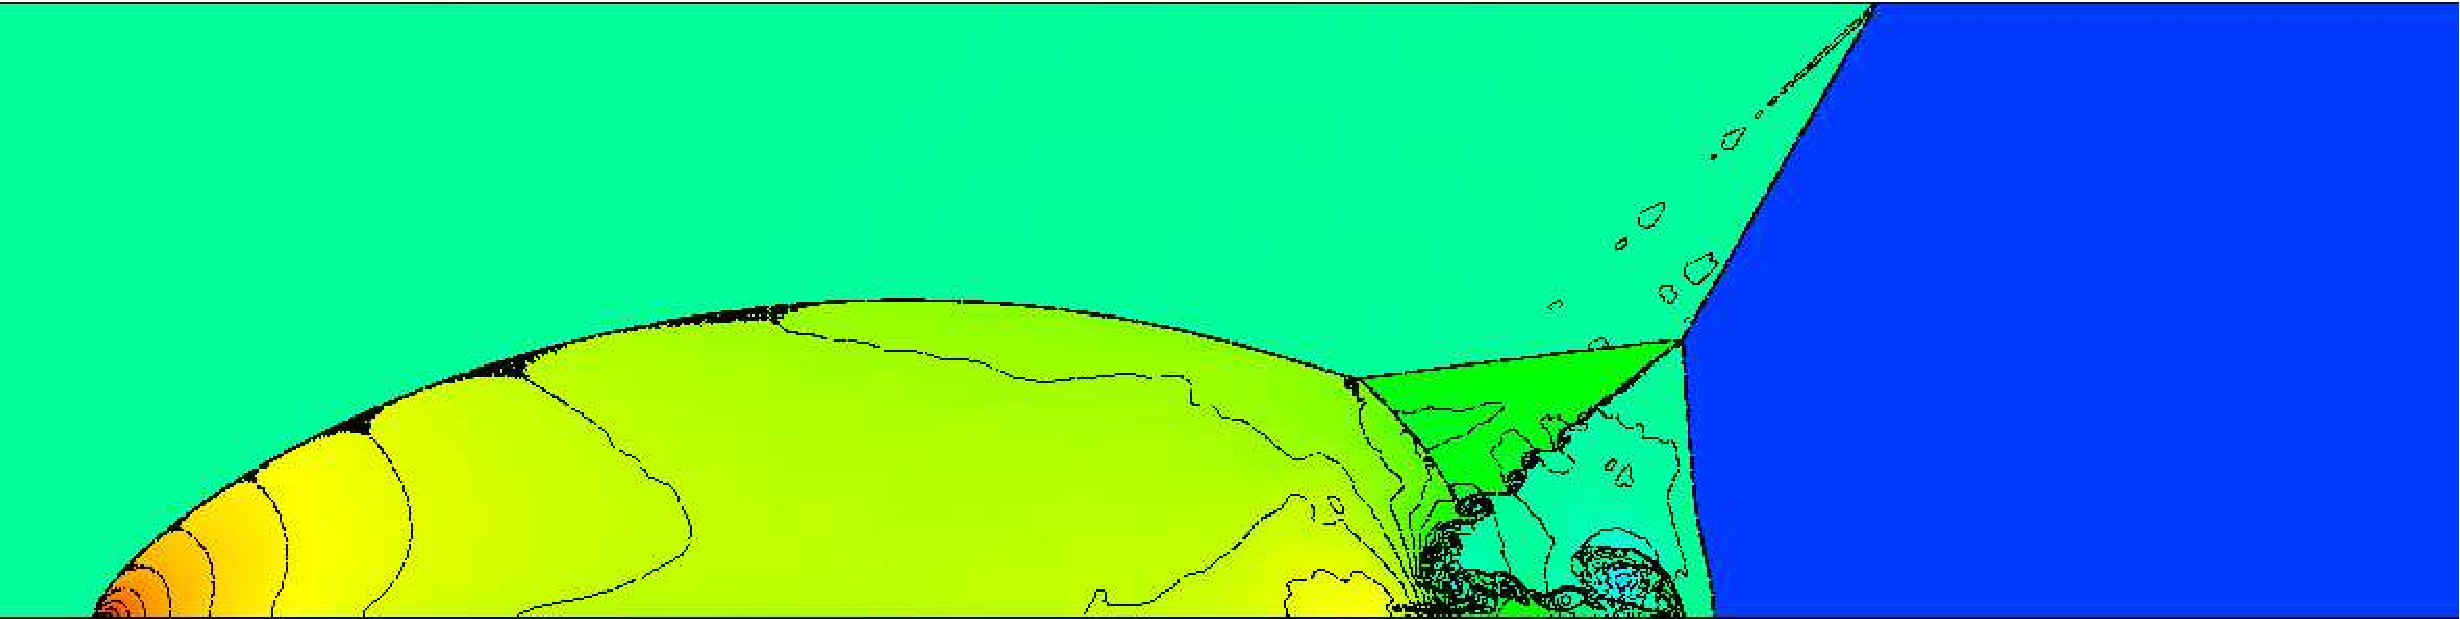
\includegraphics[width=0.9\textwidth]{dmr}
\caption{
Isopycnics for double Mach reflection, parameters are $\alpha$=60$^{\circ~}$, $\gamma$=1.4, M=10. 
This compares well with published results using this test \citep{1984jcp_woodward_colella, 1992ApJS...80..753S, 1989JCoPh..82...64B}.
Main features visible include the contact discontinuity roll-up along the lower right of the image, launching a jet of dense material towards the Mach stem and causing it to bulge outwards, the triple point or lambda point where the three shocks meet and the wall heating error where the perfect resolution at the a priori boundary condition contrasts with the slight smearing by the numerical code.
}
\label{fig:3-2} % Give a unique label
\end{figure}


\begin{figure}[t]
\centering
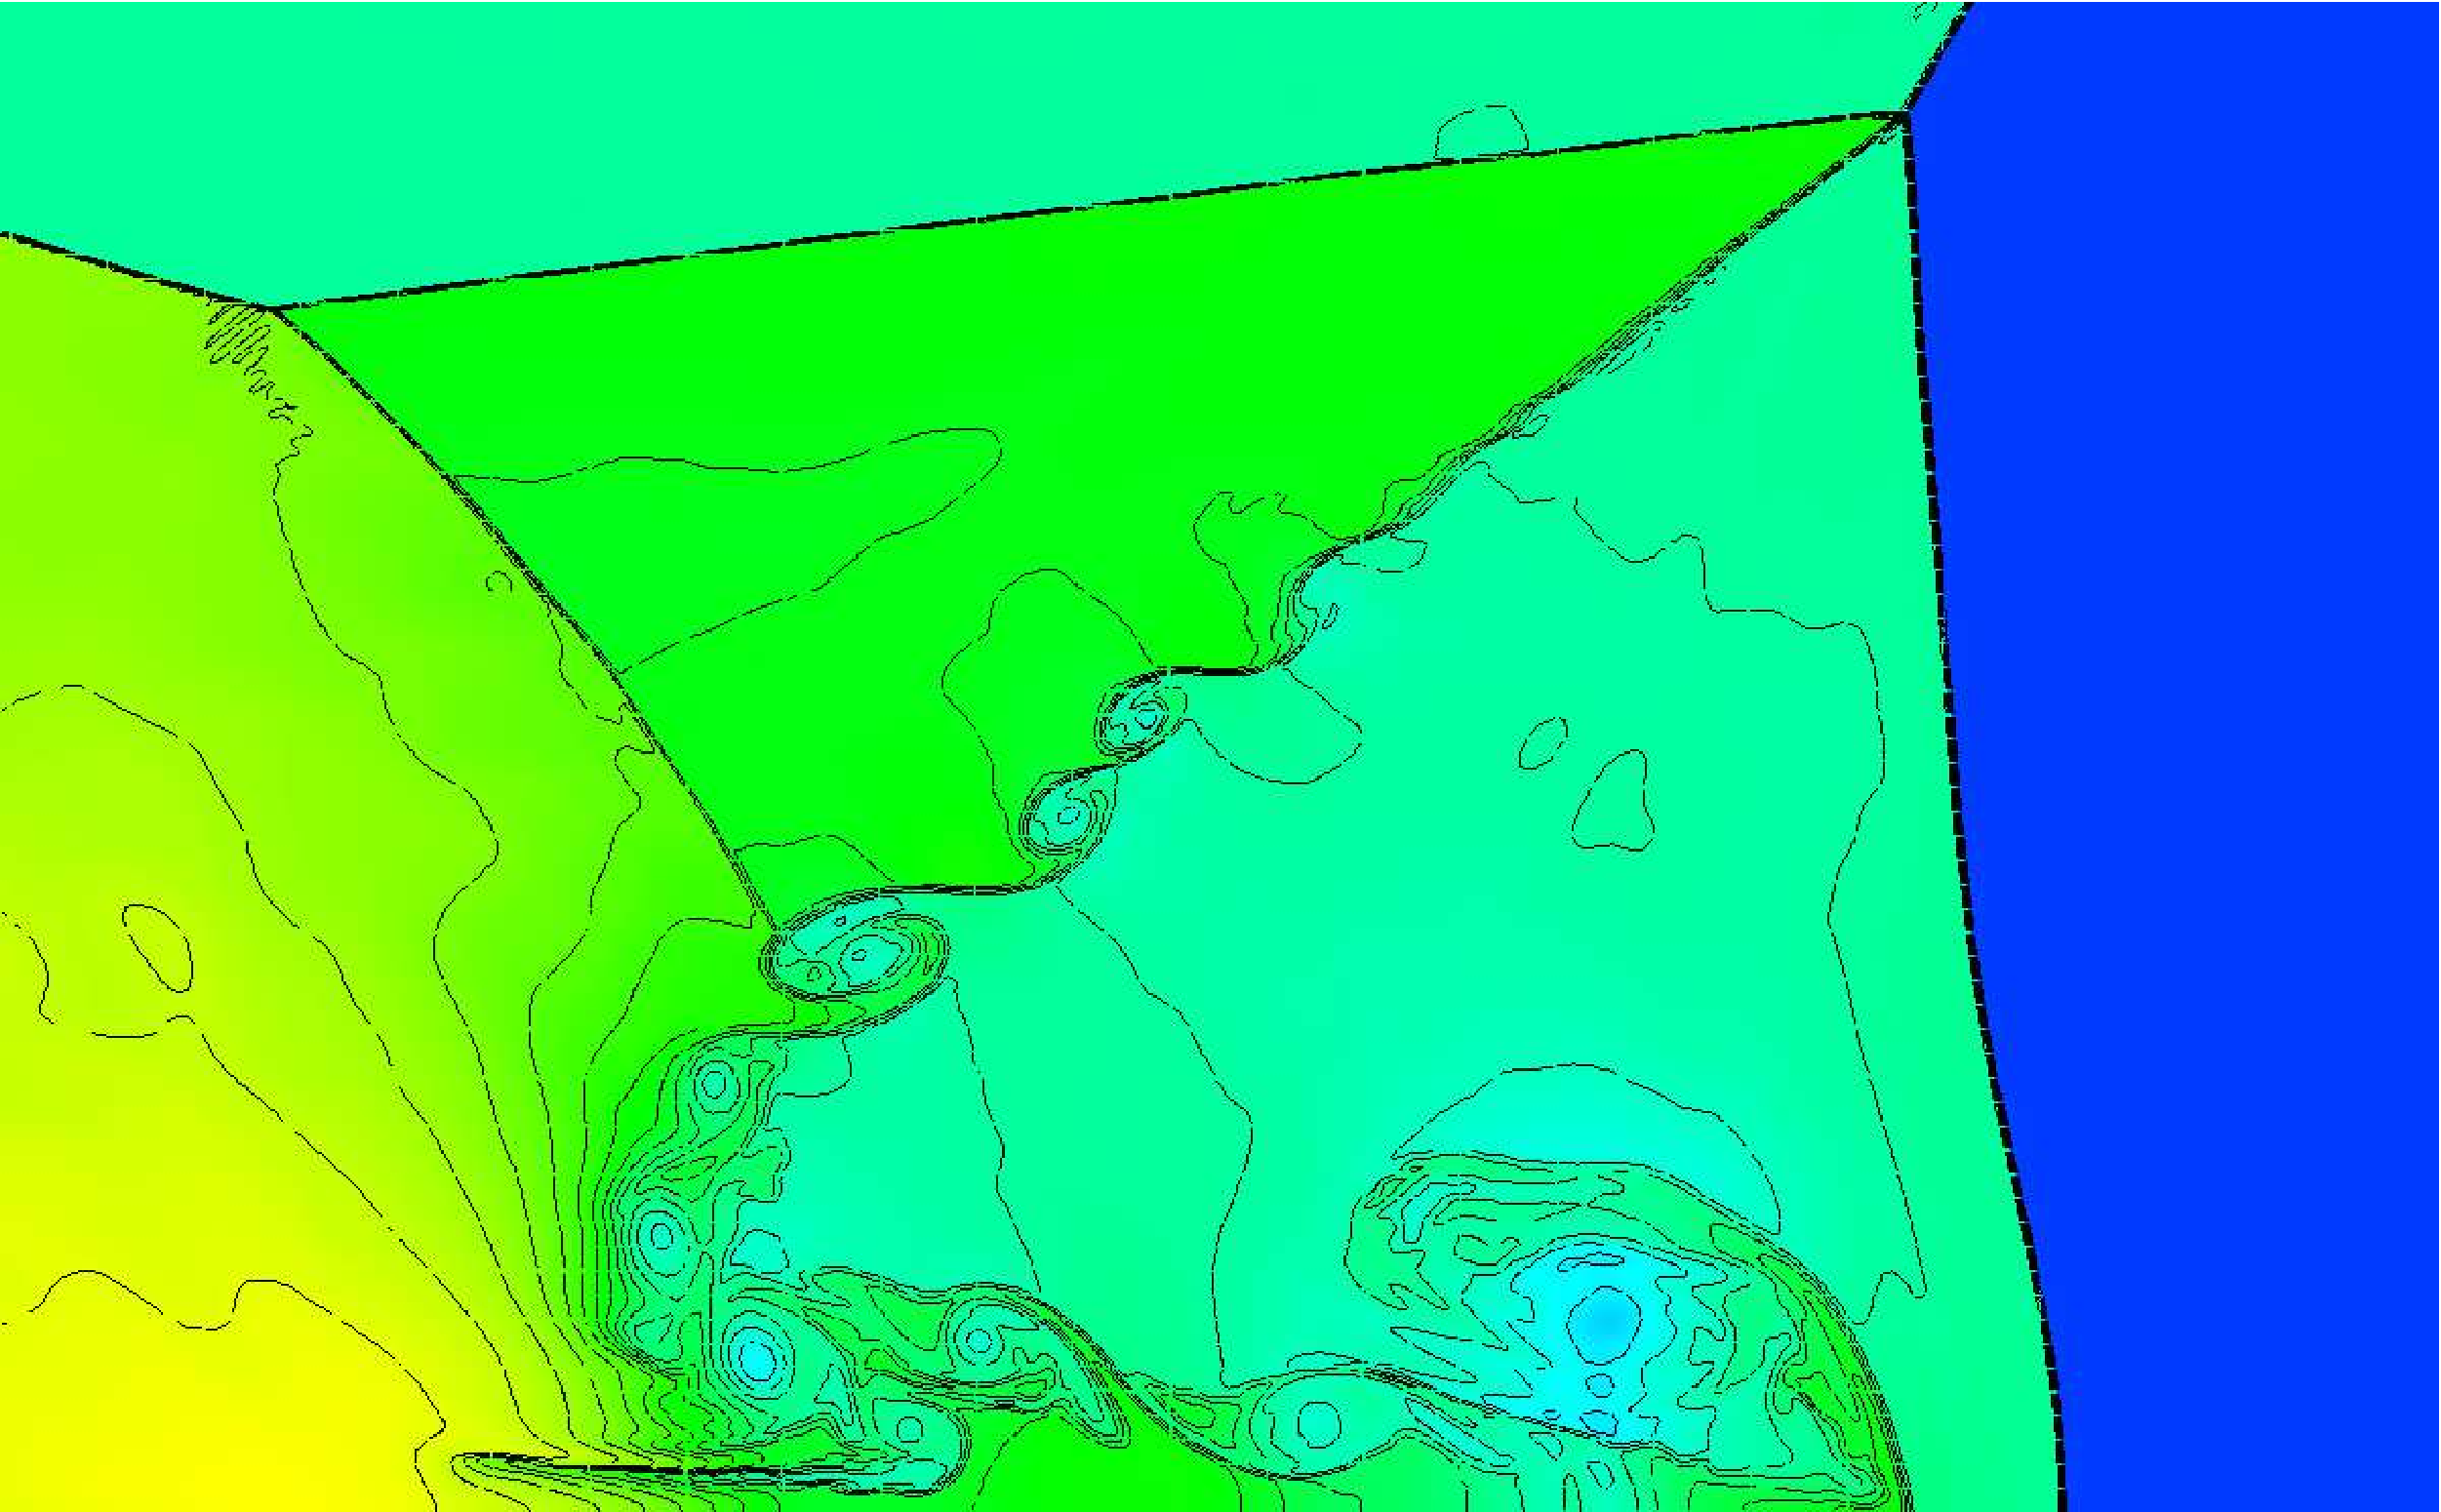
\includegraphics[width=8cm]{kh2}
\caption{
Isopycnics for double Mach reflection. 
Detail of Figure \ref{fig:3-2} - notice the Kelvin-Helmholtz instability on the contact discontinuity.
The triple points are evident at the upper left and right corners of the image.
The jet of dense material which causes the Mach stem to bulge outwards is also visible.
}
\label{fig:3-3} % Give a unique label
\end{figure}

\section{Cooling Tests}
\subsection{Overstable Radiative Shock}

% want to test radiative cooling and see if it behaves in accordance with theory.
%To test the radiative cooling and see if it behaves in accordance with theory,
%one popular test is to see if it shows the oscillations which signify the overstable radiative shock.

Under certain conditions, fast radiatively cooling flows have been shown to be unstable \citep{1982ApJ...261..543C}, where the size of the shock oscillates significantly.
This instability turns on above a minimum pre-shock velocity and the onset and characteristics of this instability are powerful verifications of the correctness and general nature of any hydrodynamical code (
\citet{1984ApJ...276..667I},
\citet{1988ApJ...329..927G},
and \citet{1987MNRAS.224..179I}).

%\citet{1982ApJ...261..543C}
%\citet{1987MNRAS.224..179I,1987MNRAS.226...67I,1987MNRAS.227.1021I}
%to test the cooling function is working correctly.
The main characteristic, overstable oscillation occurs when a shock moving away from a wall increases its cooling length so has a larger cooling region. 
The shock loses thermal pressure support and falls back towards the wall, which then repressurises it and drives it back out again.
% wrong xxxx After approximately one cooling length the shock will have been slowed down by the cooling and will weaken and fall backwards towards the wall, which then repressurises the shock and drives it back out again, and the cycle continues \citep{1988ApJ...329..927G}.



\begin{figure}[t]
\centering
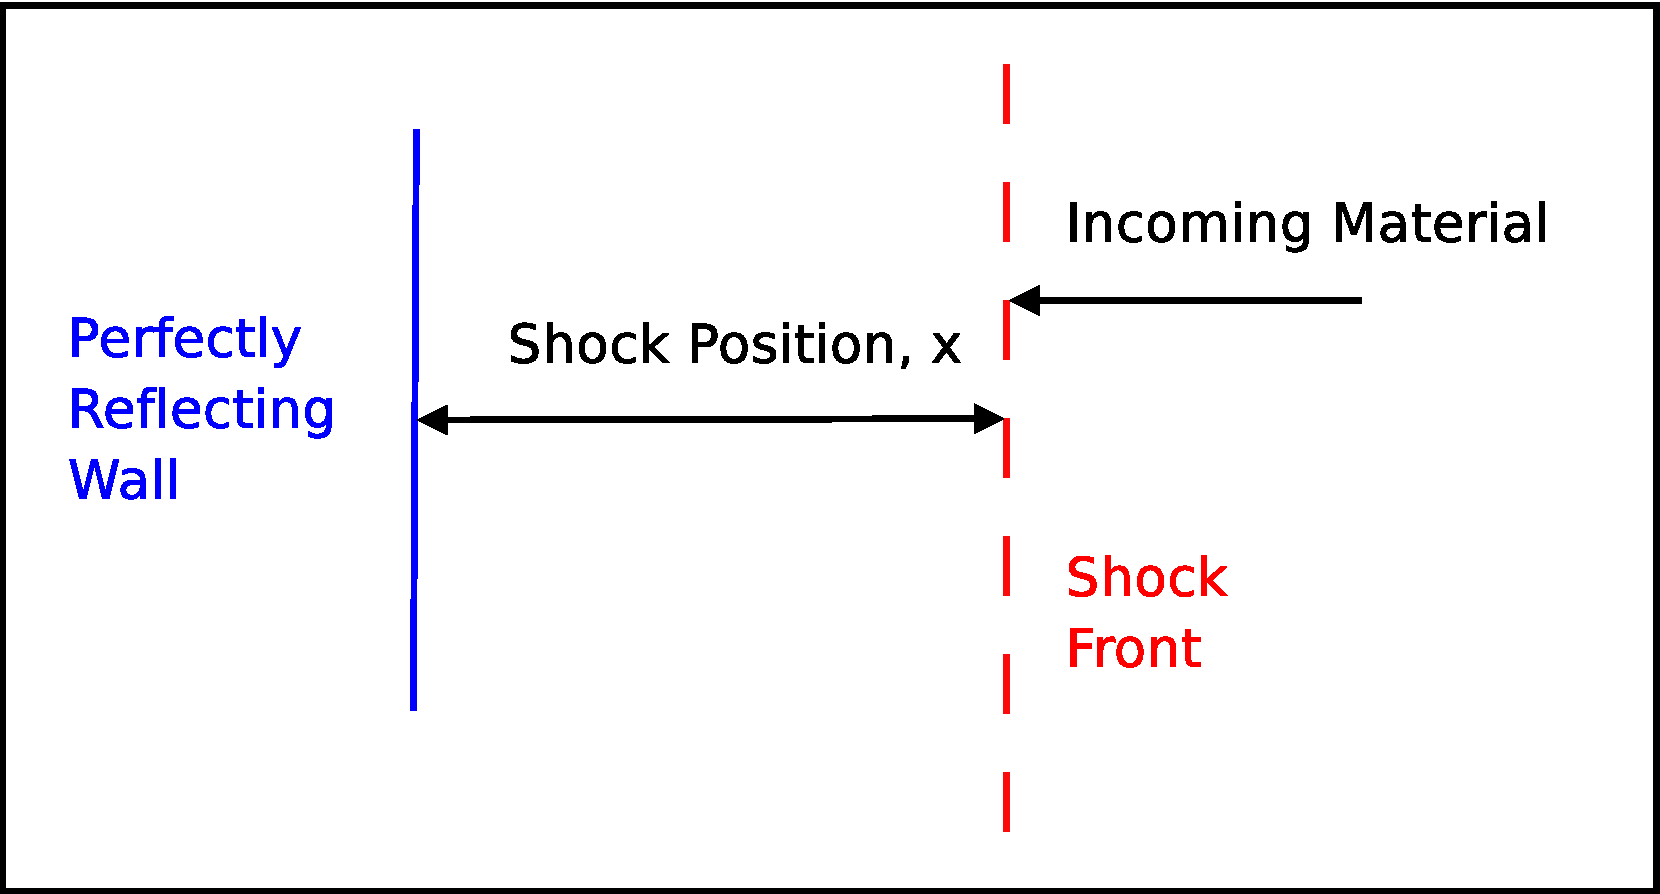
\includegraphics[width=8cm]{OverStableShockSchematic}
\caption{
Strong radiative shock reflected from a wall, oscillating back and forth.
}
\label{fig:OverStableShockSchematic} % Give a unique label
\end{figure}

\begin{figure}[t]
\centering
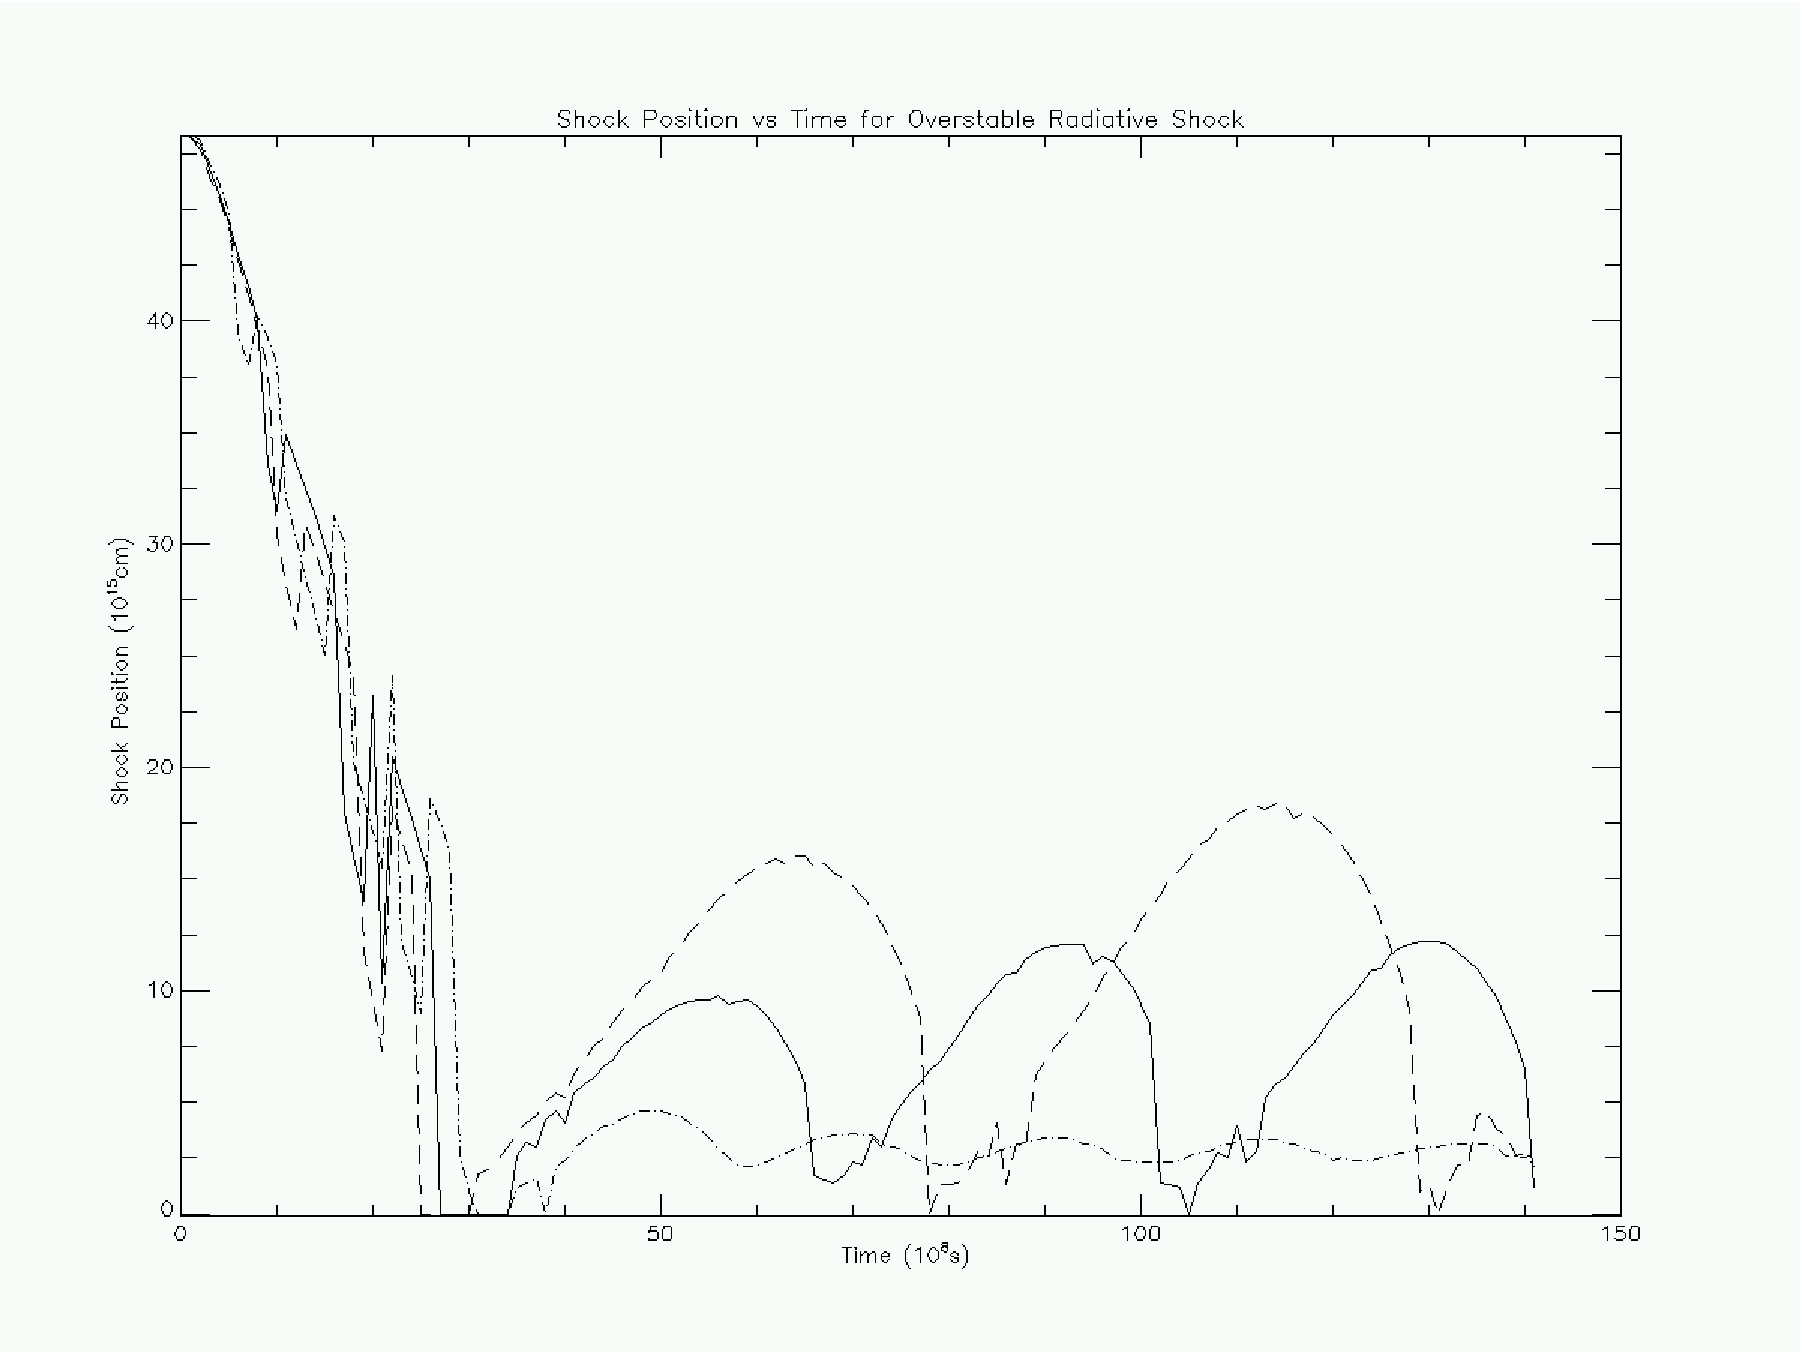
\includegraphics[width=8cm]{osrshock}
\caption{
Shock position vs. time plotted for overstable radiative shock test, for velocities, 140, 160, 170 km/s.
The results shown for velocities of 140, 160 and 170 km/s demonstrate that the stability limit lies in the range below 140 km/s.
}
\label{fig:3-6} % Give a unique label
\end{figure}


The results shown for velocities of 140,160 and 170 km/s demonstrate that the stability limit lies in the range below 140 km/s.

\section{MHD Tests}
\subsection{MHD Shock Tube}



\begin{figure*}[tb]
  \centering
  %GNUPLOT: LaTeX picture with Postscript
\begin{picture}(0,0)%
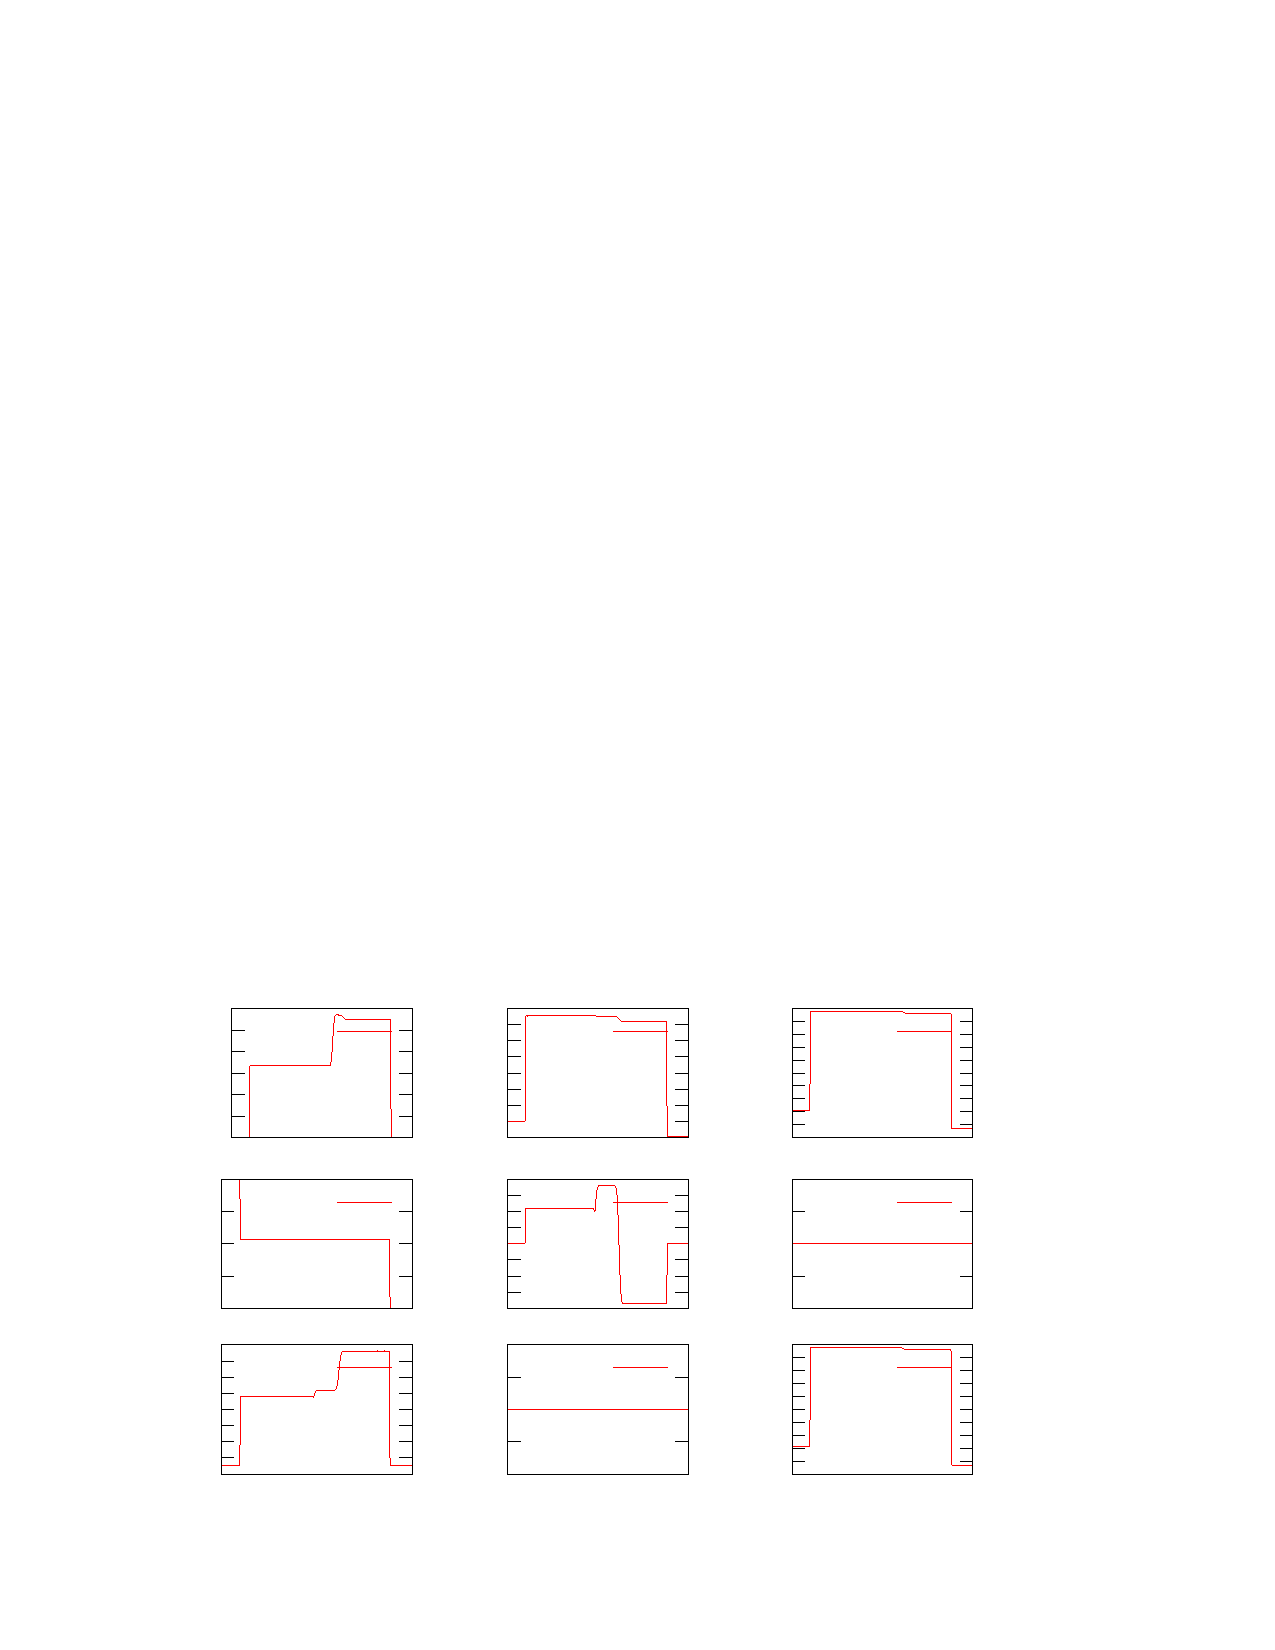
\includegraphics{epslatex/rj1a}%
\end{picture}%
\begingroup
\setlength{\unitlength}{0.0200bp}%
\begin{picture}(20699,12419)(0,0)%
\put(1707,8697){\makebox(0,0)[r]{\strut{} 1}}%
\put(1707,9214){\makebox(0,0)[r]{\strut{} 1.5}}%
\put(1707,9730){\makebox(0,0)[r]{\strut{} 2}}%
\put(1707,10247){\makebox(0,0)[r]{\strut{} 2.5}}%
\put(1707,10763){\makebox(0,0)[r]{\strut{} 3}}%
\put(1707,11280){\makebox(0,0)[r]{\strut{} 3.5}}%
\put(1707,11796){\makebox(0,0)[r]{\strut{} 4}}%
\put(4238,11246){\makebox(0,0)[r]{\strut{}$\rho$}}%
\put(8331,8697){\makebox(0,0)[r]{\strut{} 0}}%
\put(8331,9084){\makebox(0,0)[r]{\strut{} 20}}%
\put(8331,9472){\makebox(0,0)[r]{\strut{} 40}}%
\put(8331,9859){\makebox(0,0)[r]{\strut{} 60}}%
\put(8331,10246){\makebox(0,0)[r]{\strut{} 80}}%
\put(8331,10634){\makebox(0,0)[r]{\strut{} 100}}%
\put(8331,11021){\makebox(0,0)[r]{\strut{} 120}}%
\put(8331,11409){\makebox(0,0)[r]{\strut{} 140}}%
\put(8331,11796){\makebox(0,0)[r]{\strut{} 160}}%
\put(10862,11246){\makebox(0,0)[r]{\strut{}$p_g$}}%
\put(15162,8697){\makebox(0,0)[r]{\strut{} 40}}%
\put(15162,9007){\makebox(0,0)[r]{\strut{} 60}}%
\put(15162,9317){\makebox(0,0)[r]{\strut{} 80}}%
\put(15162,9627){\makebox(0,0)[r]{\strut{} 100}}%
\put(15162,9937){\makebox(0,0)[r]{\strut{} 120}}%
\put(15162,10246){\makebox(0,0)[r]{\strut{} 140}}%
\put(15162,10556){\makebox(0,0)[r]{\strut{} 160}}%
\put(15162,10866){\makebox(0,0)[r]{\strut{} 180}}%
\put(15162,11176){\makebox(0,0)[r]{\strut{} 200}}%
\put(15162,11486){\makebox(0,0)[r]{\strut{} 220}}%
\put(15162,11796){\makebox(0,0)[r]{\strut{} 240}}%
\put(17693,11246){\makebox(0,0)[r]{\strut{}E}}%
\put(1457,4599){\makebox(0,0)[r]{\strut{}-10}}%
\put(1457,5374){\makebox(0,0)[r]{\strut{}-5}}%
\put(1457,6148){\makebox(0,0)[r]{\strut{} 0}}%
\put(1457,6923){\makebox(0,0)[r]{\strut{} 5}}%
\put(1457,7697){\makebox(0,0)[r]{\strut{} 10}}%
\put(4238,7147){\makebox(0,0)[r]{\strut{}V$_x$}}%
\put(8331,4599){\makebox(0,0)[r]{\strut{}-0.4}}%
\put(8331,4986){\makebox(0,0)[r]{\strut{}-0.3}}%
\put(8331,5373){\makebox(0,0)[r]{\strut{}-0.2}}%
\put(8331,5761){\makebox(0,0)[r]{\strut{}-0.1}}%
\put(8331,6148){\makebox(0,0)[r]{\strut{} 0}}%
\put(8331,6535){\makebox(0,0)[r]{\strut{} 0.1}}%
\put(8331,6923){\makebox(0,0)[r]{\strut{} 0.2}}%
\put(8331,7310){\makebox(0,0)[r]{\strut{} 0.3}}%
\put(8331,7697){\makebox(0,0)[r]{\strut{} 0.4}}%
\put(10862,7147){\makebox(0,0)[r]{\strut{}V$_y$}}%
\put(15162,4599){\makebox(0,0)[r]{\strut{}-1}}%
\put(15162,5374){\makebox(0,0)[r]{\strut{}-0.5}}%
\put(15162,6148){\makebox(0,0)[r]{\strut{} 0}}%
\put(15162,6923){\makebox(0,0)[r]{\strut{} 0.5}}%
\put(15162,7697){\makebox(0,0)[r]{\strut{} 1}}%
\put(17693,7147){\makebox(0,0)[r]{\strut{}V$_z$}}%
\put(1457,624){\makebox(0,0)[r]{\strut{} 4}}%
\put(1457,1011){\makebox(0,0)[r]{\strut{} 6}}%
\put(1457,1399){\makebox(0,0)[r]{\strut{} 8}}%
\put(1457,1786){\makebox(0,0)[r]{\strut{} 10}}%
\put(1457,2174){\makebox(0,0)[r]{\strut{} 12}}%
\put(1457,2561){\makebox(0,0)[r]{\strut{} 14}}%
\put(1457,2948){\makebox(0,0)[r]{\strut{} 16}}%
\put(1457,3336){\makebox(0,0)[r]{\strut{} 18}}%
\put(1457,3723){\makebox(0,0)[r]{\strut{} 20}}%
\put(4238,3173){\makebox(0,0)[r]{\strut{}B$_y$}}%
\put(8331,624){\makebox(0,0)[r]{\strut{}-1}}%
\put(8331,1399){\makebox(0,0)[r]{\strut{}-0.5}}%
\put(8331,2174){\makebox(0,0)[r]{\strut{} 0}}%
\put(8331,2948){\makebox(0,0)[r]{\strut{} 0.5}}%
\put(8331,3723){\makebox(0,0)[r]{\strut{} 1}}%
\put(10862,3173){\makebox(0,0)[r]{\strut{}B$_z$}}%
\put(15162,624){\makebox(0,0)[r]{\strut{} 40}}%
\put(15162,934){\makebox(0,0)[r]{\strut{} 60}}%
\put(15162,1244){\makebox(0,0)[r]{\strut{} 80}}%
\put(15162,1554){\makebox(0,0)[r]{\strut{} 100}}%
\put(15162,1864){\makebox(0,0)[r]{\strut{} 120}}%
\put(15162,2173){\makebox(0,0)[r]{\strut{} 140}}%
\put(15162,2483){\makebox(0,0)[r]{\strut{} 160}}%
\put(15162,2793){\makebox(0,0)[r]{\strut{} 180}}%
\put(15162,3103){\makebox(0,0)[r]{\strut{} 200}}%
\put(15162,3413){\makebox(0,0)[r]{\strut{} 220}}%
\put(15162,3723){\makebox(0,0)[r]{\strut{} 240}}%
\put(17693,3173){\makebox(0,0)[r]{\strut{}$\phi$}}%
\end{picture}%
\endgroup
\endinput

  \caption{Results of the first one-dimensional MHD shock tube \citet{1995ApJ...442..228R} test at time t=0.8 for comparison with \citet{1995ApJ...442..228R}.  The results of the simulation show the main features, fast shock, slow rarefaction, contact discontinuity, slow shock and fast shock have all been captured, however the contact discontinuity has been smeared over a few cells.
}
  \label{fig:rj1a}
\end{figure*}

\begin{figure*}[tb]
  \centering
  %GNUPLOT: LaTeX picture with Postscript
\begin{picture}(0,0)%
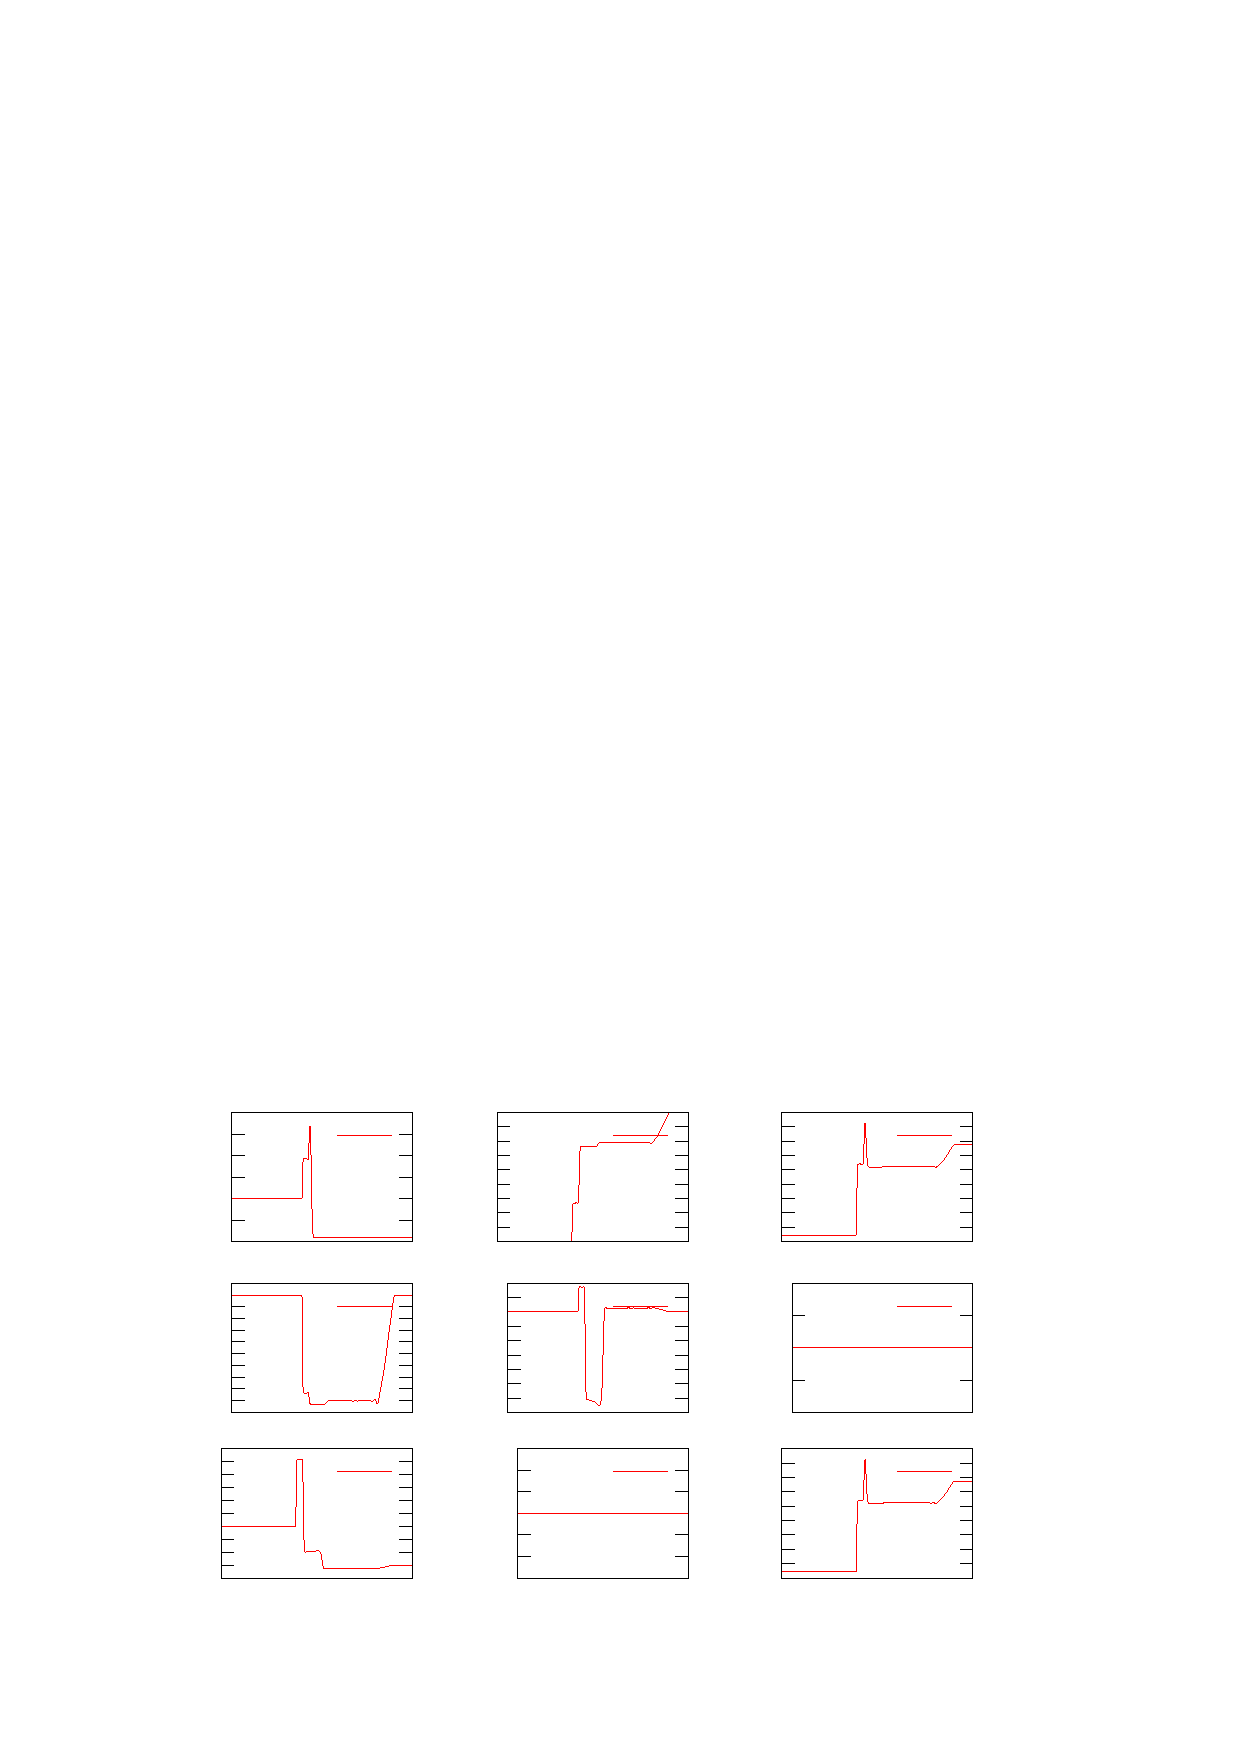
\includegraphics{epslatex/rj1b}%
\end{picture}%
\begingroup
\setlength{\unitlength}{0.0200bp}%
\begin{picture}(20699,12419)(0,0)%
\put(1707,8697){\makebox(0,0)[r]{\strut{} 0}}%
\put(1707,9214){\makebox(0,0)[r]{\strut{} 0.5}}%
\put(1707,9730){\makebox(0,0)[r]{\strut{} 1}}%
\put(1707,10247){\makebox(0,0)[r]{\strut{} 1.5}}%
\put(1707,10763){\makebox(0,0)[r]{\strut{} 2}}%
\put(1707,11280){\makebox(0,0)[r]{\strut{} 2.5}}%
\put(1707,11796){\makebox(0,0)[r]{\strut{} 3}}%
\put(4238,11246){\makebox(0,0)[r]{\strut{}$\rho$}}%
\put(8081,8697){\makebox(0,0)[r]{\strut{} 1}}%
\put(8081,9041){\makebox(0,0)[r]{\strut{} 2}}%
\put(8081,9386){\makebox(0,0)[r]{\strut{} 3}}%
\put(8081,9730){\makebox(0,0)[r]{\strut{} 4}}%
\put(8081,10074){\makebox(0,0)[r]{\strut{} 5}}%
\put(8081,10419){\makebox(0,0)[r]{\strut{} 6}}%
\put(8081,10763){\makebox(0,0)[r]{\strut{} 7}}%
\put(8081,11107){\makebox(0,0)[r]{\strut{} 8}}%
\put(8081,11452){\makebox(0,0)[r]{\strut{} 9}}%
\put(8081,11796){\makebox(0,0)[r]{\strut{} 10}}%
\put(10862,11246){\makebox(0,0)[r]{\strut{}$p_g$}}%
\put(14912,8697){\makebox(0,0)[r]{\strut{} 2}}%
\put(14912,9041){\makebox(0,0)[r]{\strut{} 4}}%
\put(14912,9386){\makebox(0,0)[r]{\strut{} 6}}%
\put(14912,9730){\makebox(0,0)[r]{\strut{} 8}}%
\put(14912,10074){\makebox(0,0)[r]{\strut{} 10}}%
\put(14912,10419){\makebox(0,0)[r]{\strut{} 12}}%
\put(14912,10763){\makebox(0,0)[r]{\strut{} 14}}%
\put(14912,11107){\makebox(0,0)[r]{\strut{} 16}}%
\put(14912,11452){\makebox(0,0)[r]{\strut{} 18}}%
\put(14912,11796){\makebox(0,0)[r]{\strut{} 20}}%
\put(17693,11246){\makebox(0,0)[r]{\strut{}E}}%
\put(1707,4599){\makebox(0,0)[r]{\strut{}-2}}%
\put(1707,4881){\makebox(0,0)[r]{\strut{}-1.8}}%
\put(1707,5162){\makebox(0,0)[r]{\strut{}-1.6}}%
\put(1707,5444){\makebox(0,0)[r]{\strut{}-1.4}}%
\put(1707,5726){\makebox(0,0)[r]{\strut{}-1.2}}%
\put(1707,6007){\makebox(0,0)[r]{\strut{}-1}}%
\put(1707,6289){\makebox(0,0)[r]{\strut{}-0.8}}%
\put(1707,6570){\makebox(0,0)[r]{\strut{}-0.6}}%
\put(1707,6852){\makebox(0,0)[r]{\strut{}-0.4}}%
\put(1707,7134){\makebox(0,0)[r]{\strut{}-0.2}}%
\put(1707,7415){\makebox(0,0)[r]{\strut{} 0}}%
\put(1707,7697){\makebox(0,0)[r]{\strut{} 0.2}}%
\put(4238,7147){\makebox(0,0)[r]{\strut{}V$_x$}}%
\put(8331,4599){\makebox(0,0)[r]{\strut{}-1.4}}%
\put(8331,4943){\makebox(0,0)[r]{\strut{}-1.2}}%
\put(8331,5287){\makebox(0,0)[r]{\strut{}-1}}%
\put(8331,5632){\makebox(0,0)[r]{\strut{}-0.8}}%
\put(8331,5976){\makebox(0,0)[r]{\strut{}-0.6}}%
\put(8331,6320){\makebox(0,0)[r]{\strut{}-0.4}}%
\put(8331,6664){\makebox(0,0)[r]{\strut{}-0.2}}%
\put(8331,7009){\makebox(0,0)[r]{\strut{} 0}}%
\put(8331,7353){\makebox(0,0)[r]{\strut{} 0.2}}%
\put(8331,7697){\makebox(0,0)[r]{\strut{} 0.4}}%
\put(10862,7147){\makebox(0,0)[r]{\strut{}V$_y$}}%
\put(15162,4599){\makebox(0,0)[r]{\strut{}-1}}%
\put(15162,5374){\makebox(0,0)[r]{\strut{}-0.5}}%
\put(15162,6148){\makebox(0,0)[r]{\strut{} 0}}%
\put(15162,6923){\makebox(0,0)[r]{\strut{} 0.5}}%
\put(15162,7697){\makebox(0,0)[r]{\strut{} 1}}%
\put(17693,7147){\makebox(0,0)[r]{\strut{}V$_z$}}%
\put(1457,624){\makebox(0,0)[r]{\strut{} 1}}%
\put(1457,934){\makebox(0,0)[r]{\strut{} 2}}%
\put(1457,1244){\makebox(0,0)[r]{\strut{} 3}}%
\put(1457,1554){\makebox(0,0)[r]{\strut{} 4}}%
\put(1457,1864){\makebox(0,0)[r]{\strut{} 5}}%
\put(1457,2173){\makebox(0,0)[r]{\strut{} 6}}%
\put(1457,2483){\makebox(0,0)[r]{\strut{} 7}}%
\put(1457,2793){\makebox(0,0)[r]{\strut{} 8}}%
\put(1457,3103){\makebox(0,0)[r]{\strut{} 9}}%
\put(1457,3413){\makebox(0,0)[r]{\strut{} 10}}%
\put(1457,3723){\makebox(0,0)[r]{\strut{} 11}}%
\put(4238,3173){\makebox(0,0)[r]{\strut{}B$_y$}}%
\put(8581,624){\makebox(0,0)[r]{\strut{} 2.97}}%
\put(8581,1140){\makebox(0,0)[r]{\strut{} 2.98}}%
\put(8581,1657){\makebox(0,0)[r]{\strut{} 2.99}}%
\put(8581,2173){\makebox(0,0)[r]{\strut{} 3}}%
\put(8581,2690){\makebox(0,0)[r]{\strut{} 3.01}}%
\put(8581,3206){\makebox(0,0)[r]{\strut{} 3.02}}%
\put(8581,3723){\makebox(0,0)[r]{\strut{} 3.03}}%
\put(10862,3173){\makebox(0,0)[r]{\strut{}B$_z$}}%
\put(14912,624){\makebox(0,0)[r]{\strut{} 2}}%
\put(14912,968){\makebox(0,0)[r]{\strut{} 4}}%
\put(14912,1313){\makebox(0,0)[r]{\strut{} 6}}%
\put(14912,1657){\makebox(0,0)[r]{\strut{} 8}}%
\put(14912,2001){\makebox(0,0)[r]{\strut{} 10}}%
\put(14912,2346){\makebox(0,0)[r]{\strut{} 12}}%
\put(14912,2690){\makebox(0,0)[r]{\strut{} 14}}%
\put(14912,3034){\makebox(0,0)[r]{\strut{} 16}}%
\put(14912,3379){\makebox(0,0)[r]{\strut{} 18}}%
\put(14912,3723){\makebox(0,0)[r]{\strut{} 20}}%
\put(17693,3173){\makebox(0,0)[r]{\strut{}$\phi$}}%
\end{picture}%
\endgroup
\endinput

  \caption{Results of the second one-dimensional MHD shock tube \citet{1995ApJ...442..228R} test at time t=0.8 for comparison with \citet{1995ApJ...442..228R}.  The results of the simulation show the main features, fast shock, slow slock, contact discontinuity, slow rarefaction and fast rarefaction have all been captured, however the contact discontinuity and slow shockhave been smeared over a few cells. There are also some small oscillations near the fast rarefaction (at the extreme right).
}
  \label{fig:rj1b}
\end{figure*}

Shock tube tests from \citet{1995ApJ...442..228R} are used.
All shock tube tests were carried out using a grid of 500 cells, a Courant number of 0.5 and an adiabatic index of $\gamma=5/3$.
Note that the adaptive mesh refinement is turned off so that the results can be compared with non-AMR codes. 

The initial conditions for the MHD shock tube test are as follows:
\\Left State:
\begin{equation}
U_L = \left( 
\rho = 1,
v_x =0,
v_y = 10,
p = 20,
B_x = 5,
B_y = 5
\right)
\end{equation}
\\Right State:
\begin{equation}
U_R = \left( 
\rho = 1,
v_x = 1,
v_y = -10,
p = 1,
B_x = 5,
B_y = 5
\right)
\end{equation}


The results of the simulation show the main features, fast shock, slow rarefaction, contact discontinuity, slow shock and fast shock have all been captured, however the contact discontinuity has been smeared over a few cells (see Figure \ref{fig:rj1a}).
% this is a common problem with all shock capturing schemes


The initial conditions for the second MHD shock tube test are as follows:
\\Left State:
\begin{equation}
U_L = \left( 
\rho = 1,
v_x =0,
v_y = 0,
p = 1,
B_x = 3,
B_y = 5
\right)
\end{equation}
\\Right State:
\begin{equation}
U_R = \left( 
\rho = 0.1,
v_x = 0,
v_y = 0,
p = 10,
B_x = 3,
B_y = 2
\right)
\end{equation}
The results of the simulation show the main features, fast shock, slow shock, contact discontinuity, slow rarefaction and fast rarefaction have all been captured, there is a small oscillation near the fast rarefaction (see Figure \ref{fig:rj1b}).

\subsection{Orszag-Tang Vortex}

It is more difficult to find experimental results for regimes where the ideal MHD approximations apply.
In this test a pure mathematical abstraction is used,
to test the ability of the code to respond to oblique 2D MHD shocks during the decay to into MHD turbulence.
The vortex of Orszag and Tang \citep{1979JFM....90..129O} is an excellent test of MHD shocks. 
It consists of a superposition of sinusoids of magnetic and velocity fields of different frequencies. 
It is a common test for 2D MHD (it is referred to as ``frequently touted'' in \citet{2006ApJS..165..188H} ) and has been used by among others 
\cite{2000ApJ...530..508L}, \citet{1999osullivan}, \cite{1998ApJ...494..317D}, \cite{1998ApJ...509..244R}, \citet{1995ApJ...452..785R}.
The initial conditions are taken from \citet{1999osullivan}
\begin{equation}
U = \left( 
\begin{array}{c}
\rho = \frac{25}{36\pi} \\
v_x = -\mathrm{sin}(2\pi y)\\
v_y = \mathrm{sin}(2\pi x)\\
v_z = 0\\
B_x = -\mathrm{sin}(2\pi y)\\
B_y = \mathrm{sin}(4\pi x)\\
B_z = 0\\
p = \frac{5}{12\pi}
\end{array}
\right)
\end{equation}

Values for $p$, $\rho$, and $\gamma$ are deliberately chosen, so that the speed of sound, $c=\sqrt{\gamma p/\rho}=1$.
Orszag-Tang tests how a code handles MHD shocks in the transition to 2D MHD turbulence.


\begin{figure}[t]
\centering
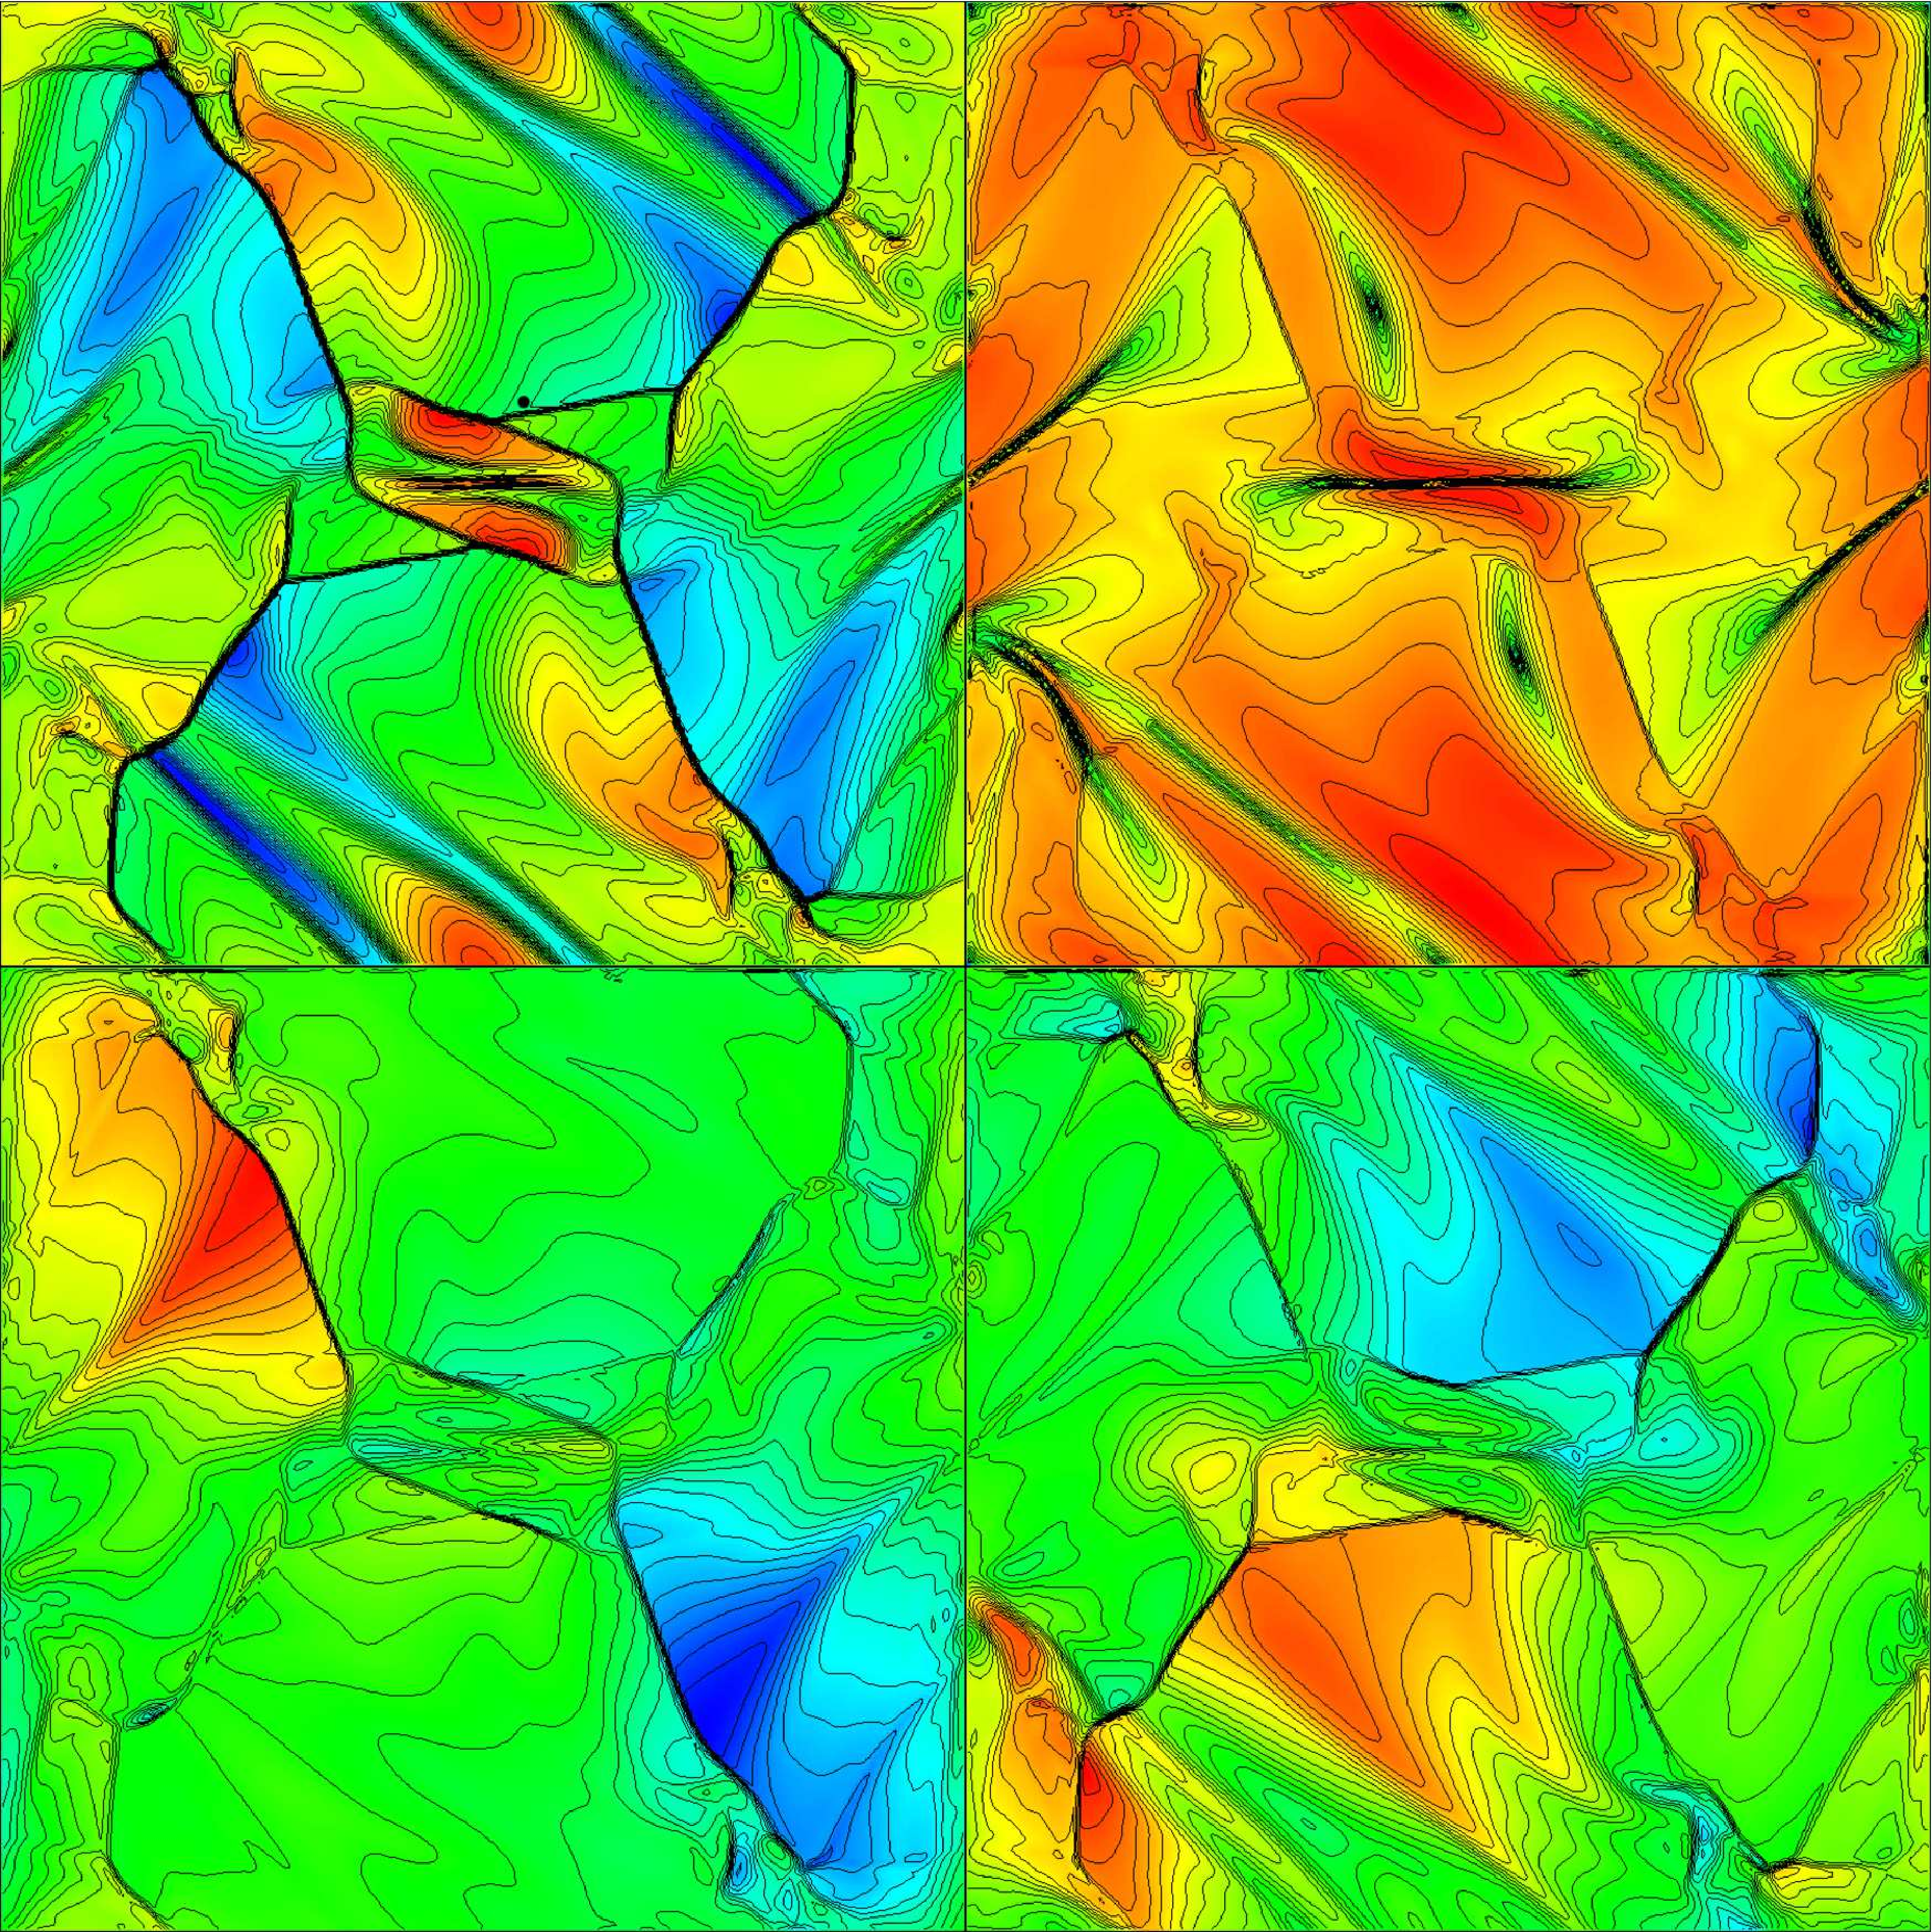
\includegraphics[width=0.6\textwidth]{orszag}
\caption{
Contours of magnetic pressure {\it(upper left)}, thermal pressure {\it(upper right)}, compressibility $\boldsymbol{\nabla} \cdot \mathbf{v}$ {\it(lower left)} and vorticity $\boldsymbol{\nabla} \times \mathbf{v}$ {\it(lower right)}.
Periodic boundary conditions were used on a domain of x=[0,1], y=[0,1] using 256x256 cells with a Courant number of 0.5.
The initial configuration was set to match that of RJF and is 
$ \rho = \frac{25}{36\pi} ,
v_x = -\mathrm{sin}(2\pi y),
v_y = \mathrm{sin}(2\pi x),
v_z = 0,
B_x = -\mathrm{sin}(2\pi y),
B_y = \mathrm{sin}(4\pi x),
B_z = 0,
p = \frac{5}{12\pi} $
The results show excellent agreement with 
\cite{2000ApJ...530..508L}, \citet{1999osullivan}, \cite{1998ApJ...494..317D}, \cite{1998ApJ...509..244R}, \citet{1995ApJ...452..785R}.
}
\label{fig:3-8} % Give a unique label
\end{figure}

The contours shown in Figure \ref{fig:3-8} demonstrate excellent agreement with preceding studies, e.g. RJF, LDZ both show excellent agreement which represents a good validation of the code. 

\subsection{MHD Blast Wave}
In the MHD blast wave test, a circular area of high pressure is embedded within a strong magnetic field.
An explosive expansion results.
This problem has been studied as a possible model for dynamical solar
phenomenae, particularly Moreton waves and EIT waves \citep{2002ApJ...572L..99C}. See 
\citet{1999SoPh..187...89C} for a review of the topic.
\citet{Gardiner05:_an_uns} studied this problem and the initial conditions from
that paper are used in this test.
In this case the magnetic field is set at an angle of 45$^\circ$.
Initial conditions for the entire grid are set to: 
\begin{equation}
U = \left( 
\begin{array}{c}
\rho = 1 \\
v_x = 0\\
v_y = 0\\
v_z = 0\\
B_x = 10/\sqrt{(2)}\\
B_y = 10/\sqrt{(2)}\\
B_z = 0\\
p = 1
\end{array}
\right)
\end{equation}
The blast is represented by a pressure 100 times the ambient pressure.
Its initial radius is 0.125. 
The simulation was performed on a grid of unit side with periodic boundary conditions. 
The density colourmap, the log magnetic pressure and the log pressure at time
t=0.2 are shown in Figure \ref{fig:3-mhdblastwave}.
The field lines are overplotted onto the density colormap.
The maximum density is 3.32, within 1\% of the result of \citet{Gardiner05:_an_uns}.
Under the influence of the external magnetic field, the initial pressure wave
loses its spherical symmetry as it propagates through the ambient medium.
Two dense shells propagate parallel to the magnetic field (the red crescents in
the density colourmap Figure \ref{fig:3-mhdblastwave}).
Perpendicular to the magnetic field, it can be seen from Figure
\ref{fig:3-mhdblastwave} that the magnetic pressure dominates over the
blast wave, and the field lines are only mildly bent.

\begin{figure}[t]
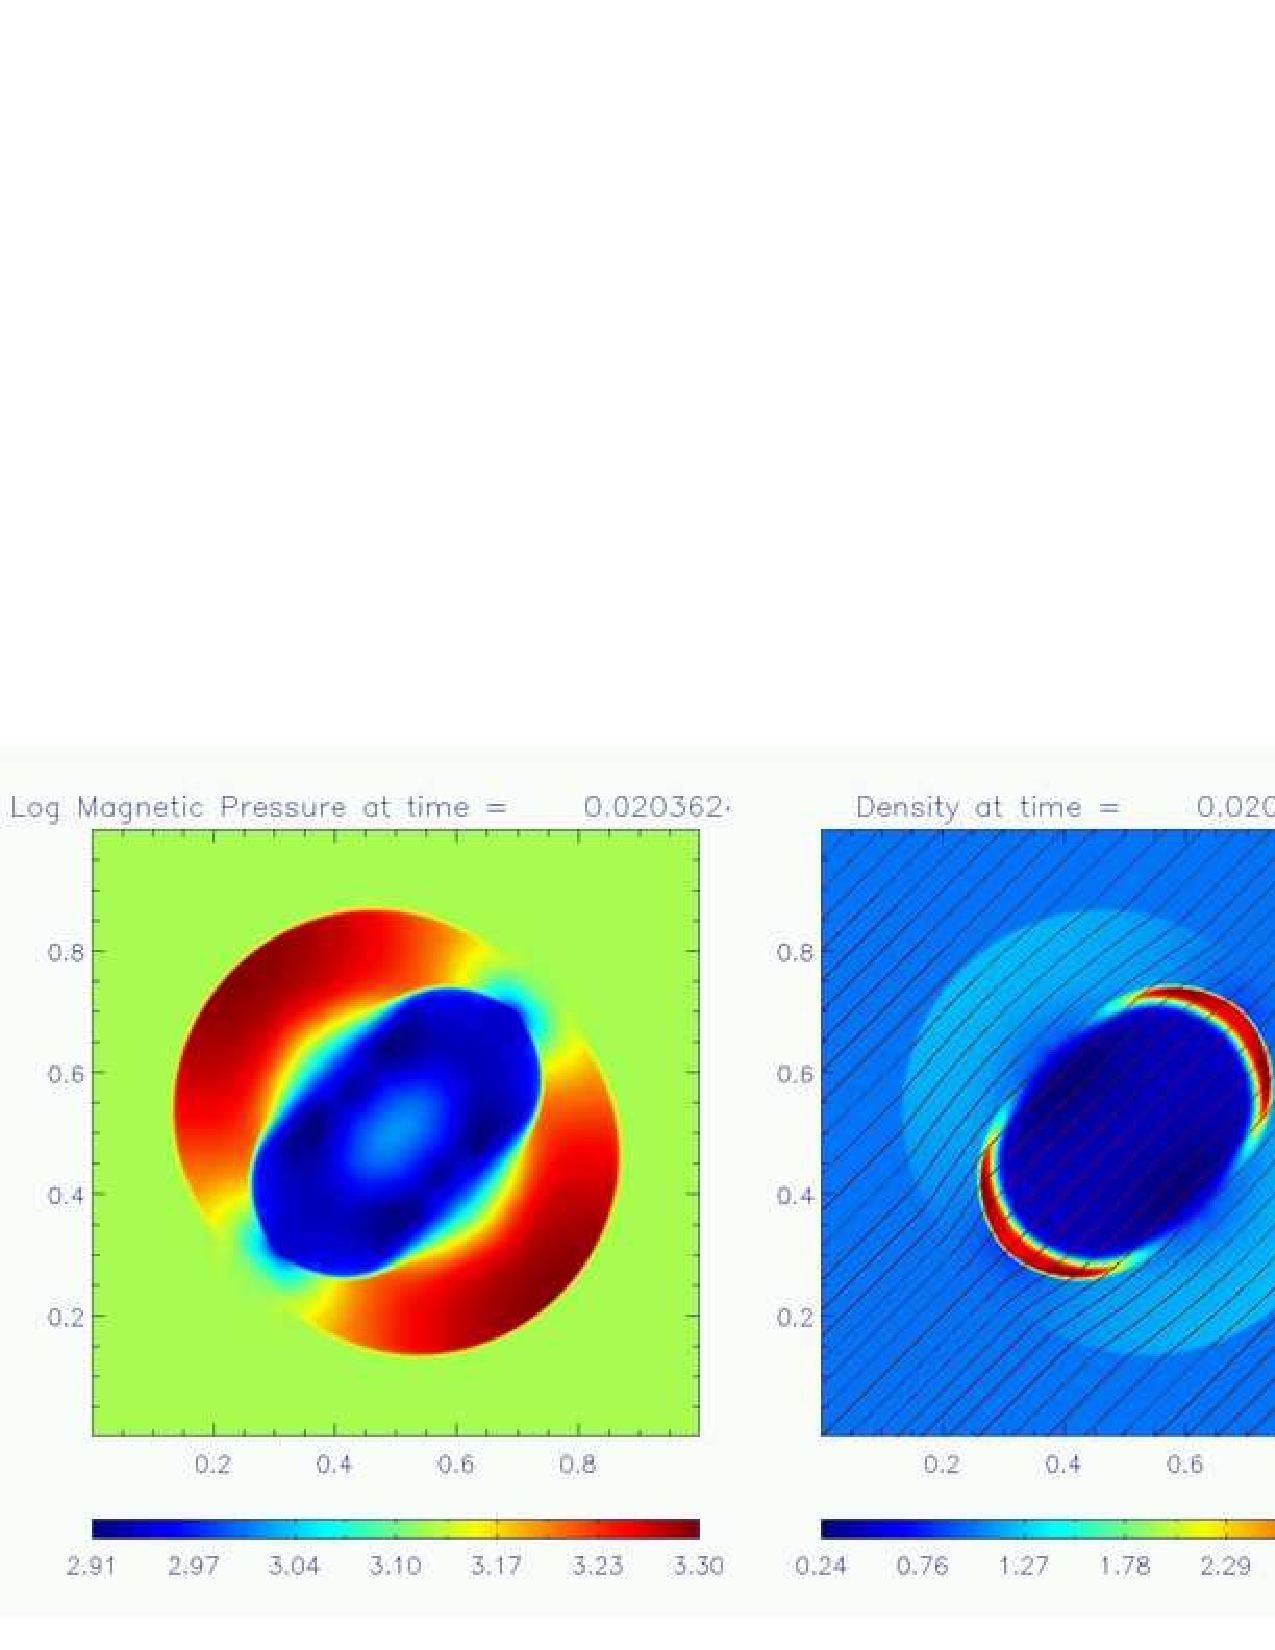
\includegraphics[width=15cm]{mhdblastwavemulti}
\caption{
Solution for the MHD blast wave log magnetic pressure, density and log thermal
pressure  at time t=0.2. The field lines are overplotted onto the density
colourmap. The initial conditions are: $\rho = 0.1, B_x = 10/\sqrt{(2)}, B_y =10/\sqrt{(2)}, p = 0.1 $.  
The grid is of unit side with periodic boundary conditions.
}
\label{fig:3-mhdblastwave} % Give a unique label
\end{figure}

\section{Simulation}
All simulations were carried out on a 32-node, 32-bit Beowulf-type cluster, Leda and on a 210-node 64-bit cluster, Rowan. 
The Fortran 90 code was compiled using the Intel optimisations for speed.

\section{Code comparison and scheme comparison}



%Comparison with the PLUTO code of A. Mignone.

In collaboration with the Torino astrophysics group a comparison of the astrophysics code ATLAS with PLUTO \citep{2004Ap&SS.293..199M} was undertaken.

\subsection{PLUTO description}
% Pluto is a modular, Godunov-type code intended mainly for astrophysical applications.  Written in C, it currently supports classical, relativistic and magneto (Newtonian and relativistic) fluid dynamics modules in Cartesian and curvilinear coordinates in 1, 2 and 3 dimensions.
% The code is particularly suitable for treating hypersonic flows with strong discontinuities, and several numerical algorithms (TVD, PPM) are available for testing. Source terms include gravity, rotations and optically thin radiative losses. Pluto works on non-uniform grids and runs either on a single processor or on parallel architectures (using MPI libraries). 
PLUTO is a versatile code which can integrate the MHD equations using the CTU method and the Roe solver. It has been used for a several jet simulations and supports Cartesian and curvilinear coordinates in 1, 2 and 3 dimensions.
The code includes implementations of several numerical algorithms in the form of modules.

\subsection{Performance}
In all tests PLUTO was noticeably faster - this is partially because the AMR in ATLAS was turned off for the purposes of the simulation and still represents some overhead.

%Several simulations were done.
%Jet pictures:
%Underdense jets
%HLLE method
%Roe method

\begin{figure}[t]
\begin{center}
\begin{minipage}[c]{.48\linewidth}
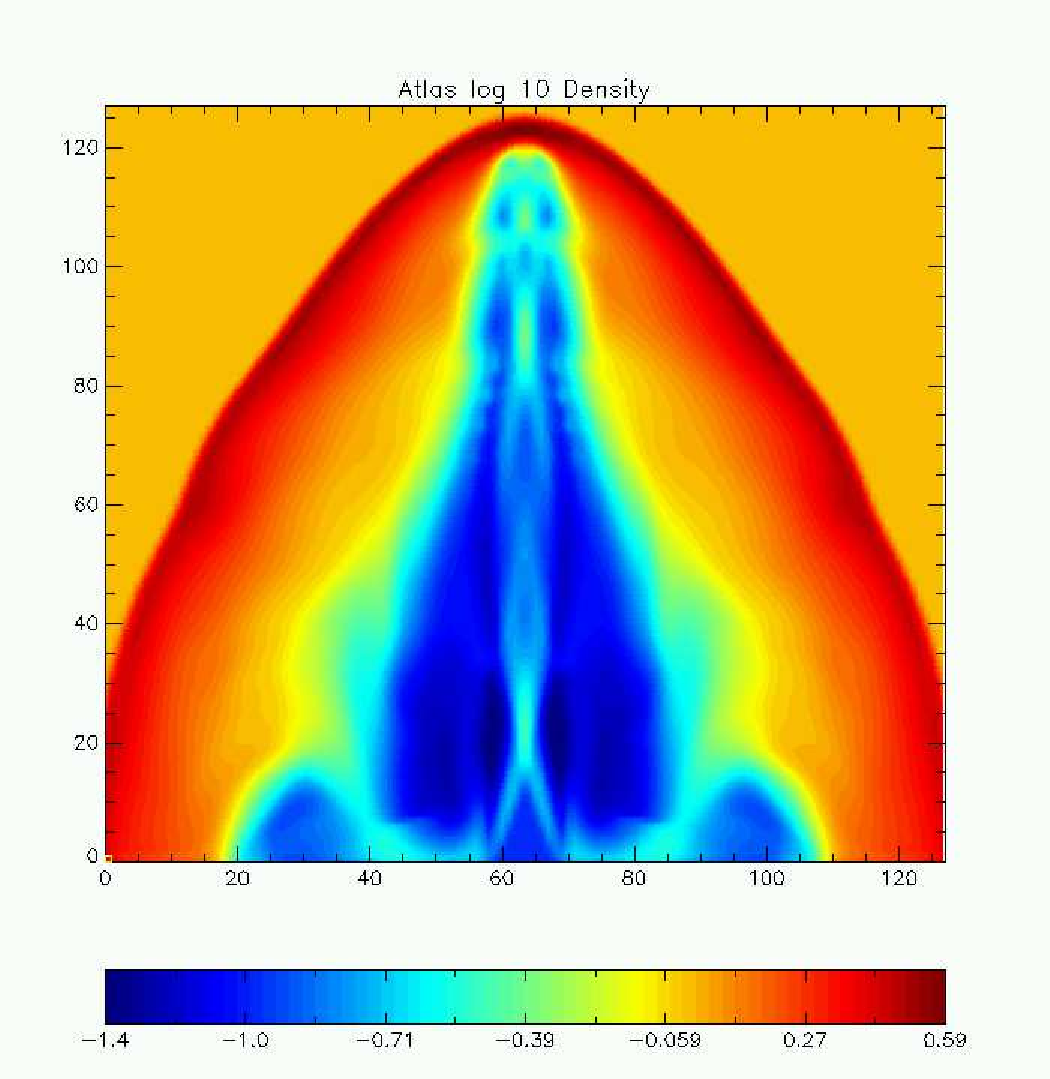
\includegraphics[width=7cm]{atlas_comparison_jet1}
\end{minipage} \hfill
\begin{minipage}[c]{.48\linewidth}
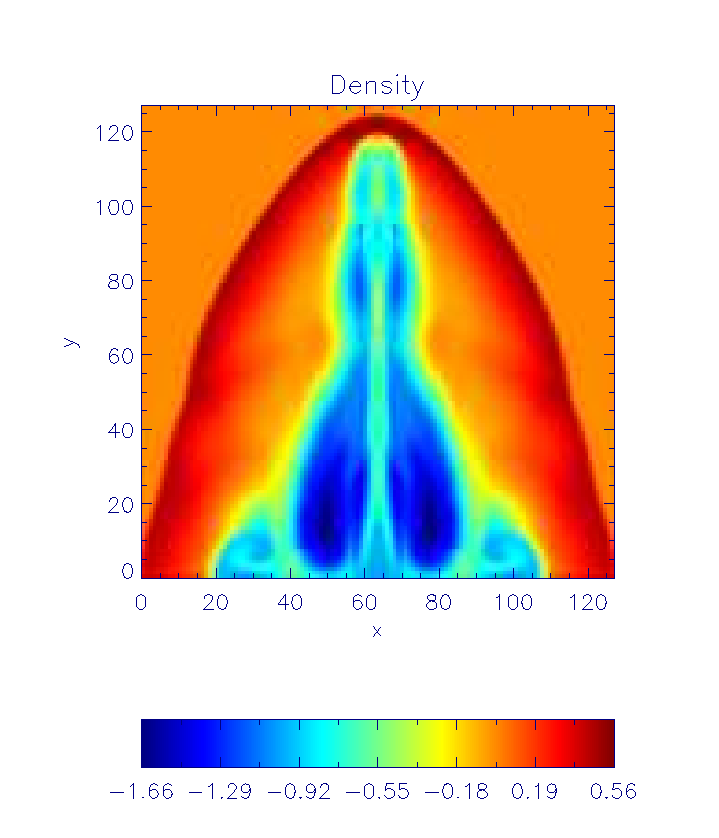
\includegraphics[width=7cm]{pluto_comparison}
\end{minipage} \hfill
\caption{
Comparison of numerical codes ATLAS and PLUTO for an underdense ($\eta=0.1$) jet, using directionally unsplit schemes and Roe solver.
}
\label{fig:compjet1} % label
\end{center}
\end{figure}

\subsection{Comparison I: Underdense Adiabatic Jet}
%There are points of similarity and difference between the two models.
The first comparison problem is an adiabatic Mach 30 jet underdense ($\eta = 0.1$) jet propagating into an undisturbed ambient medium. 
The comparison between the results shown by the two codes is shown in Figure \ref{fig:compjet1}.
As expected the jets have good agreement in speed and maximum density which agrees with the analytical result.

There are however several points of difference. The internal structure of the cocoon, the width of the bow shock and the structure of the crossing shocks along the length of the jet all show differences.

In the PLUTO simulation, two jets appear on either side of the main flow. They are much more clearly resolved than in the ATLAS solution.

%This may be an indicator that something is going wrong at the boundary.



\subsection{Comparison II: Overdense Adiabatic Jet}

\begin{figure}[t]
\begin{center}
\begin{minipage}[c]{.48\linewidth}
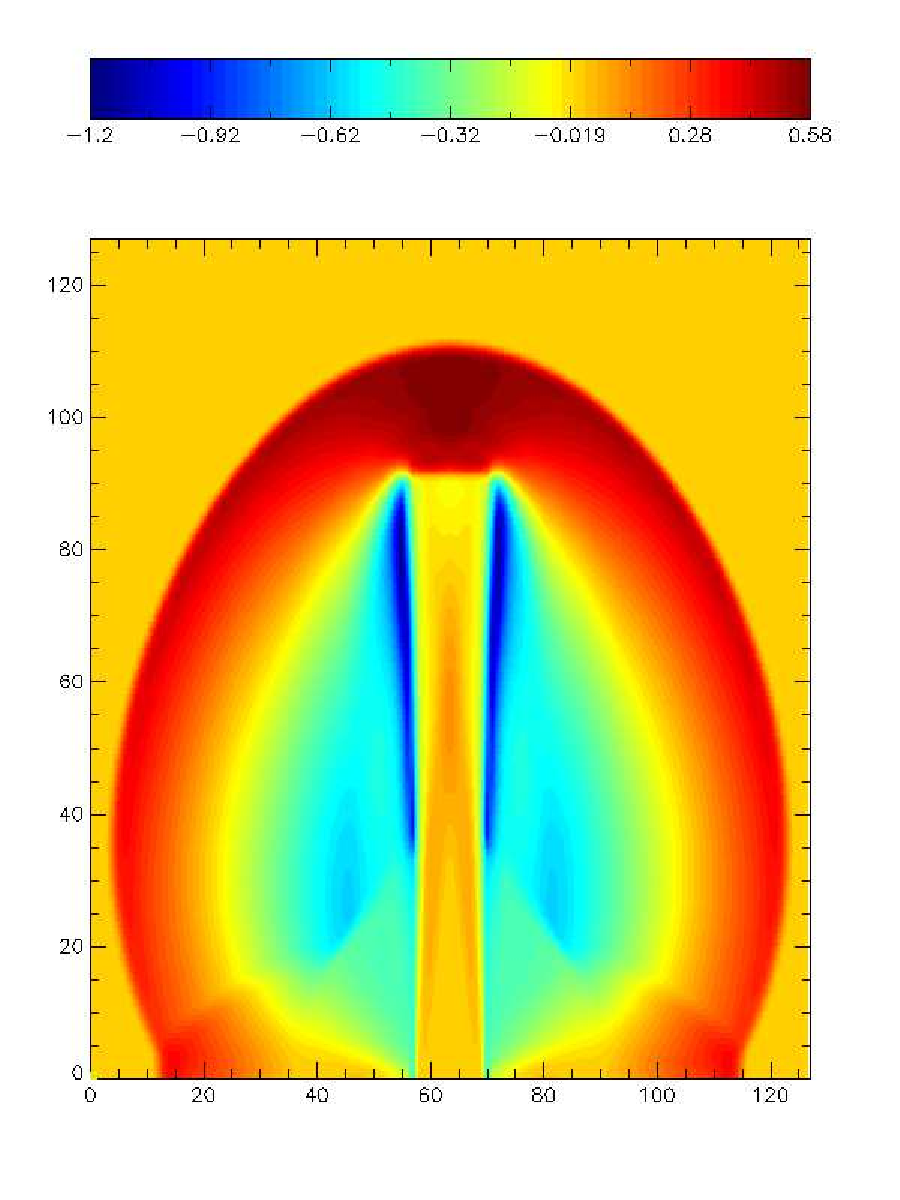
\includegraphics[width=7cm]{atlas_mach10_eta1}
\end{minipage} \hfill
\begin{minipage}[c]{.48\linewidth}
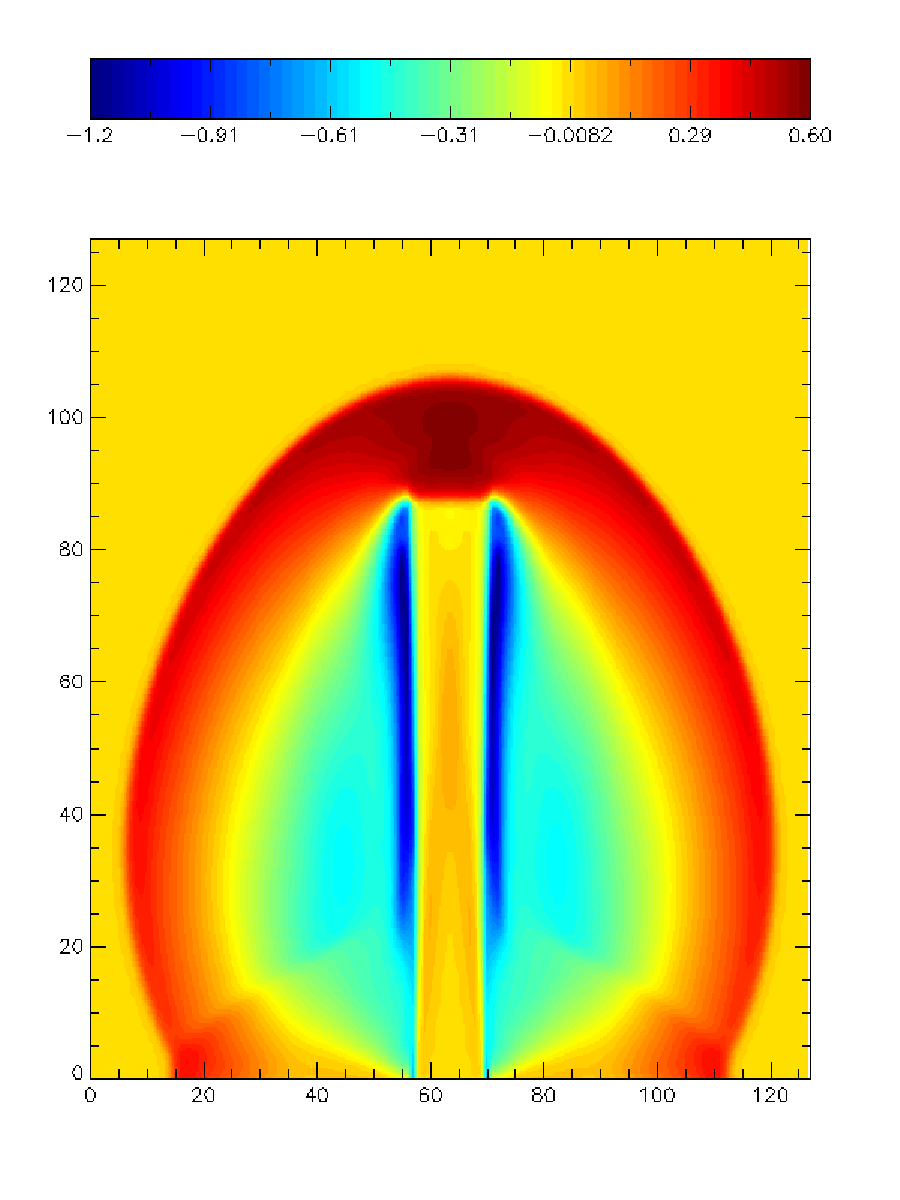
\includegraphics[width=7cm]{pluto_mach_10_eta_1}
\end{minipage} \hfill
\caption{
Density colourmaps of a comparison of numerical codes ATLAS (left panel) and PLUTO (right panel) for a Mach 10 jet, using directionally unsplit schemes and Roe solver.
}
\label{fig:compjet2} % label
\end{center}
\end{figure}

The second comparison problem is an adiabatic Mach 10 jet overdense ($\eta = 10$) jet propagating into an undisturbed ambient medium. 
The comparison between the results shown by the two codes is shown in Figure \ref{fig:compjet2}.

There are several points of similarity, the minimum densities are the same and overall appearance of the bow shock and the jet beam are very similar.

As for the points of difference, there is difference in the propagation distance
(this may be partially attributed to a slight difference in time between the two simulations)
 and the cocoon has a lower density feature in the ATLAS simulation.
In the overdense jet case there is a difference in the velocities of the two jets.
The maximum density is slightly higher in the PLUTO simulation.

The differences between the two results may result from the approximation to the spatial derivative of the conserved flux (see Section \ref{Multidimensional}), which is fourth order in PLUTO and second order in ATLAS. This results in higher order accuracy in the PLUTO result.

%REEFR code of A. Lim
%Oblique shocks closely aligned to the grid.
%Quirk
%Viscosity 
%Lapidus
%Colella viscosity

\section{Summary}
The code has been tested thoroughly in one and two dimensions and shown to be accurate and robust.
For the one-dimensional tests there is good agreement with the analytical results.
For the two-dimensional tests, qualitatively there is good agreement with experimental results, providing some level of validation to the code for these problems. Quantitatively the results agree with the published results of numerical codes.
%%Three-dimensional tests:
%Code comparison:
From the code comparison with the astrophysics code PLUTO it may be seen that there is good agreement.

